\section{Opracowane wyniki}

\subsection{Job Satisfaction Survey}

\begin{figure}[h!t]
    \centering
    \subfloat[Płaca]{\label{fig:his-pay}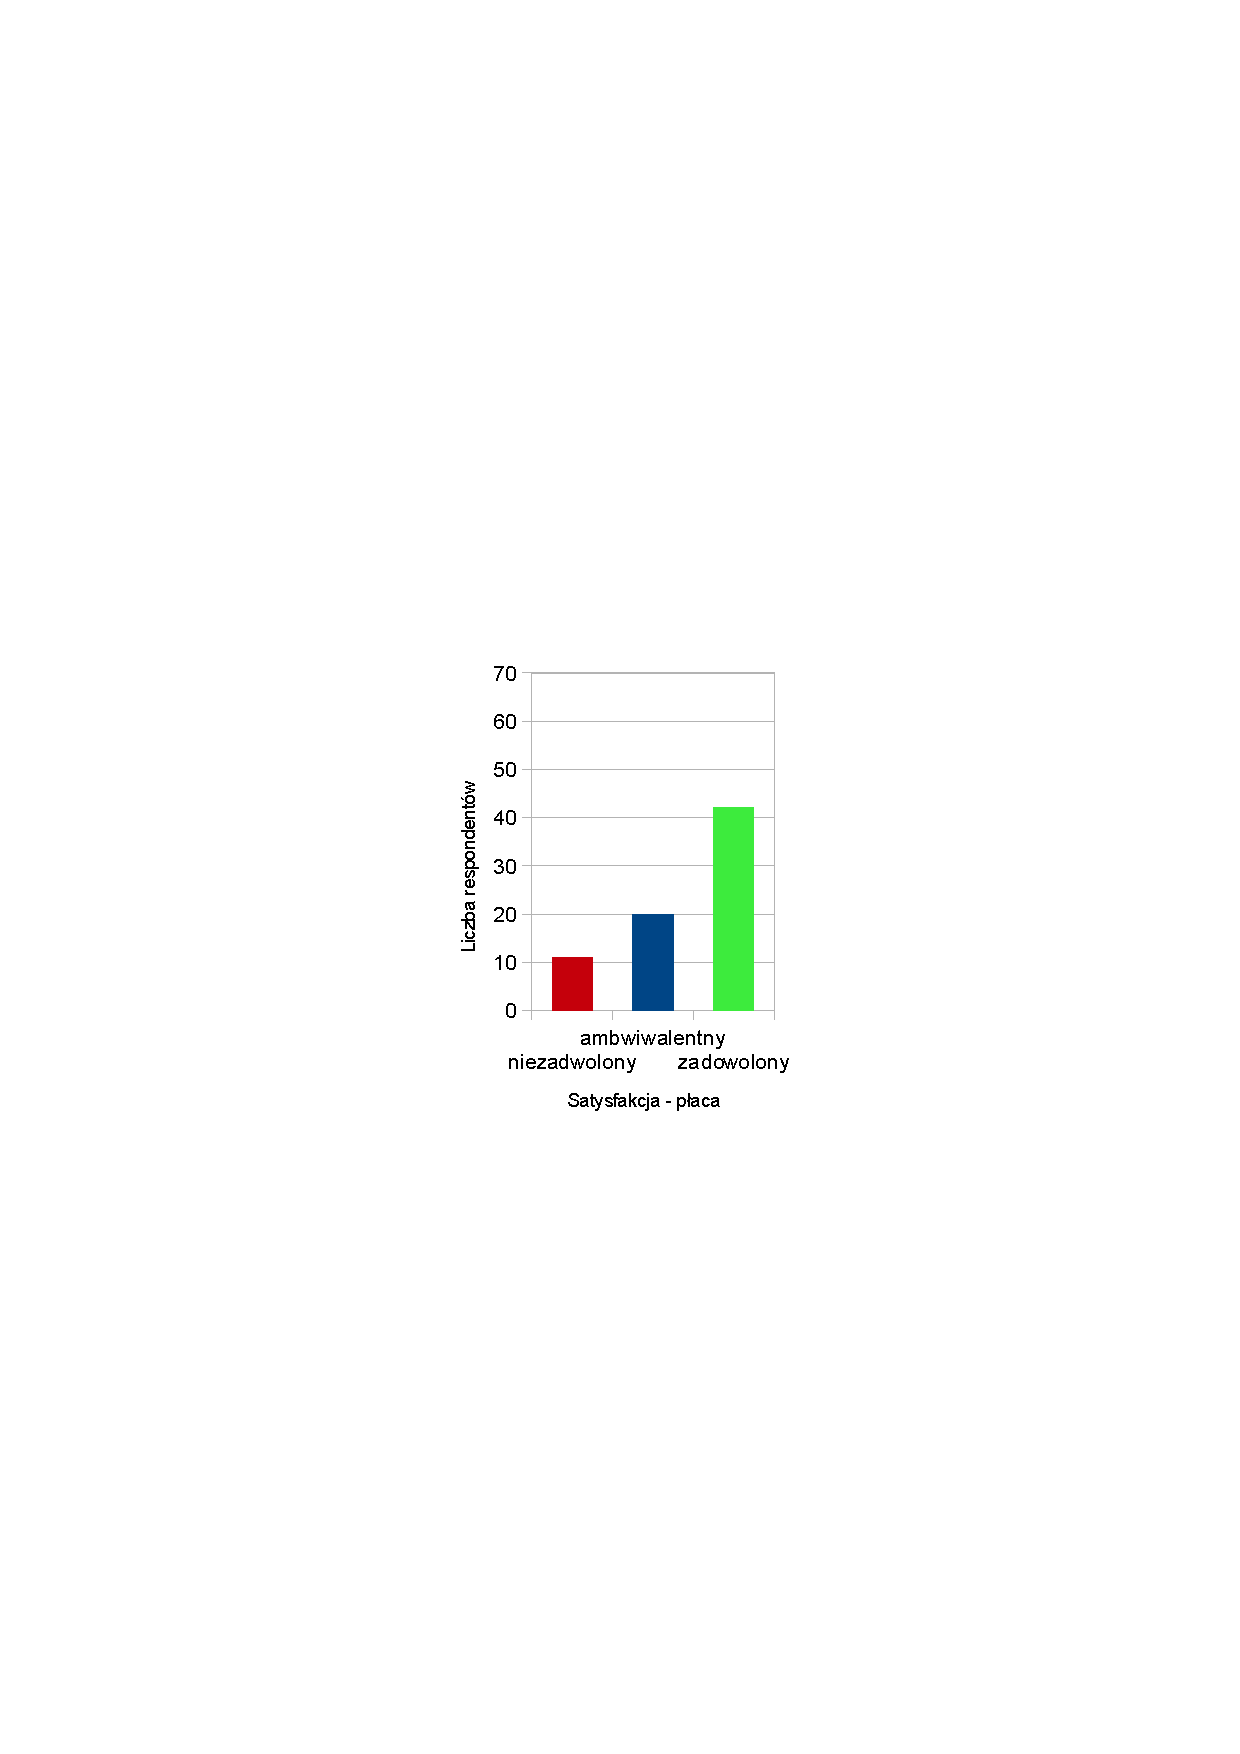
\includegraphics[height=0.27\textheight]{sat-pay}}
    \subfloat[Awanse]{\label{fig:his-promotion}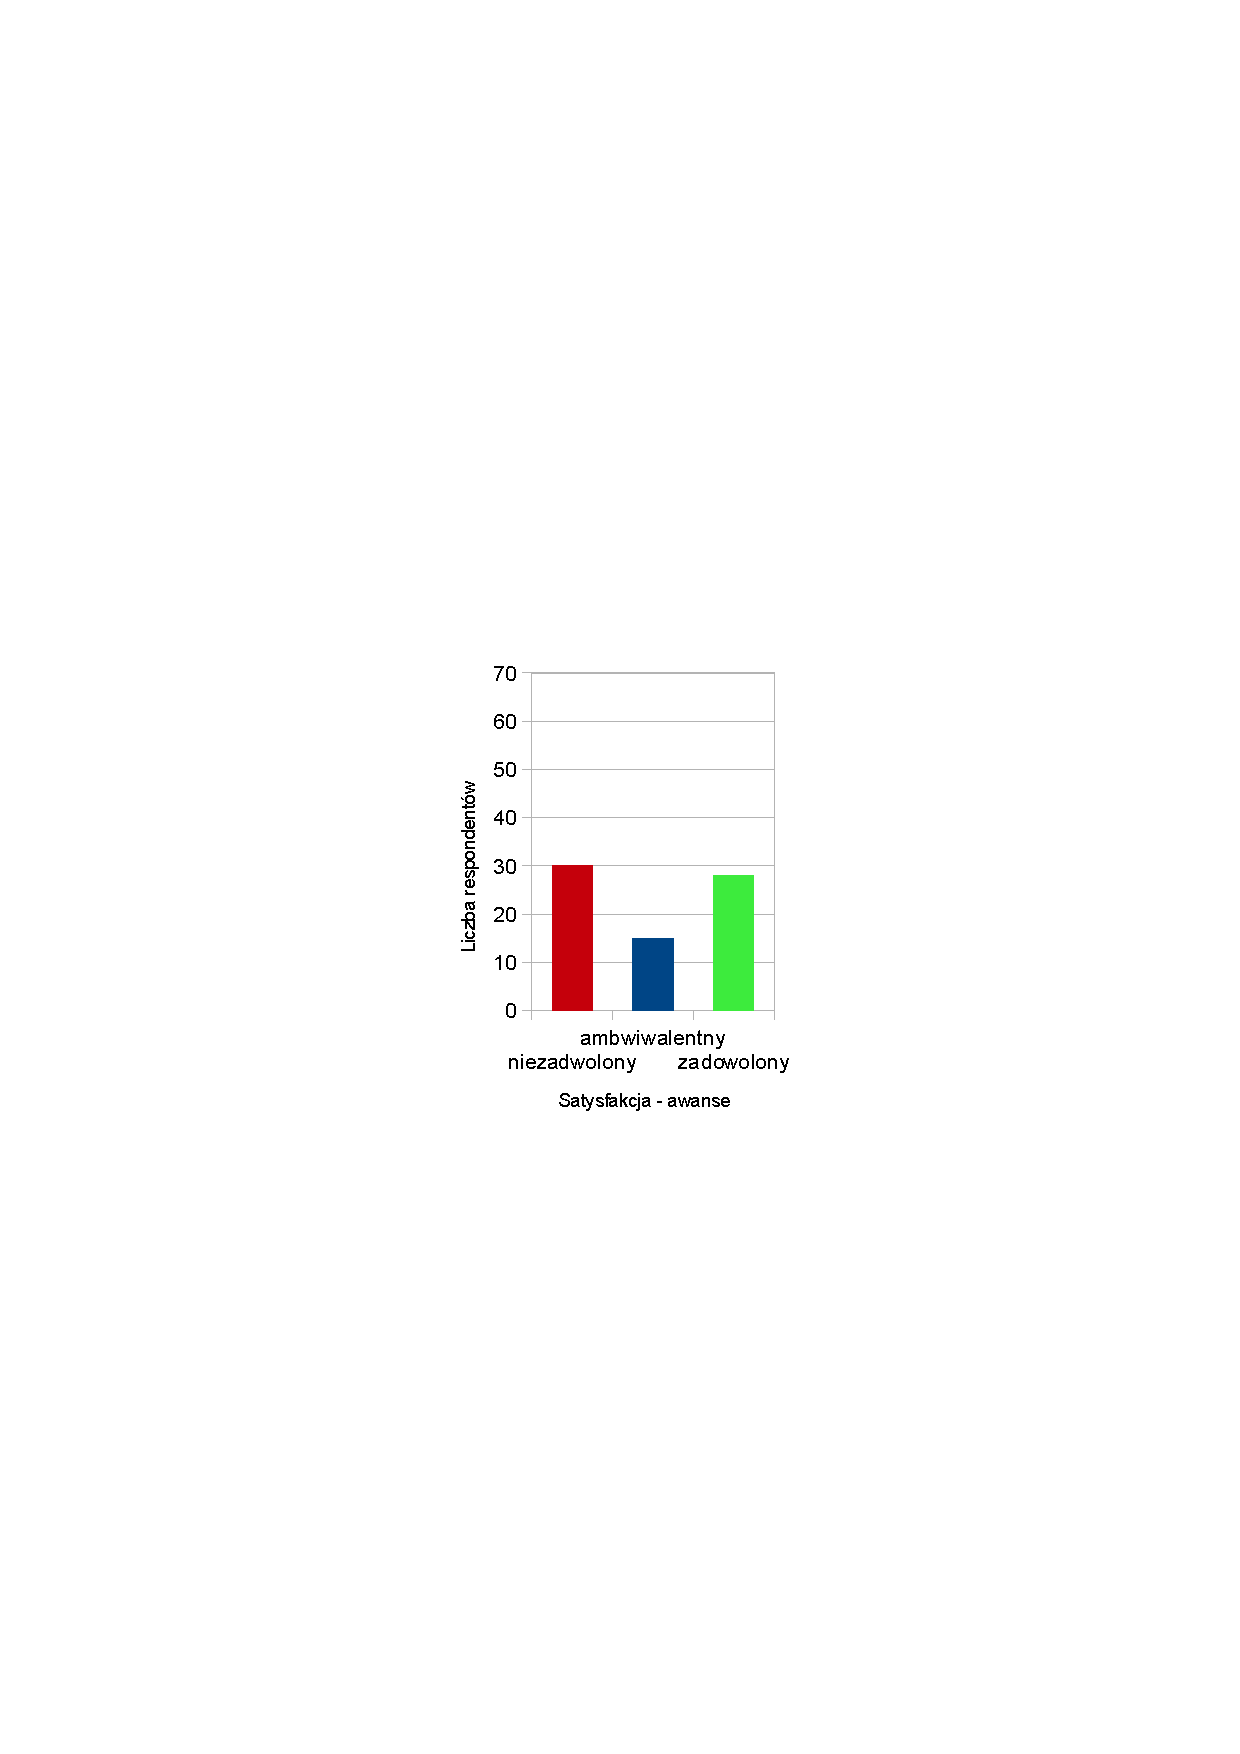
\includegraphics[height=0.27\textheight]{sat-promotion}}
    \\
    \subfloat[Nadzór]{\label{fig:his-supervision}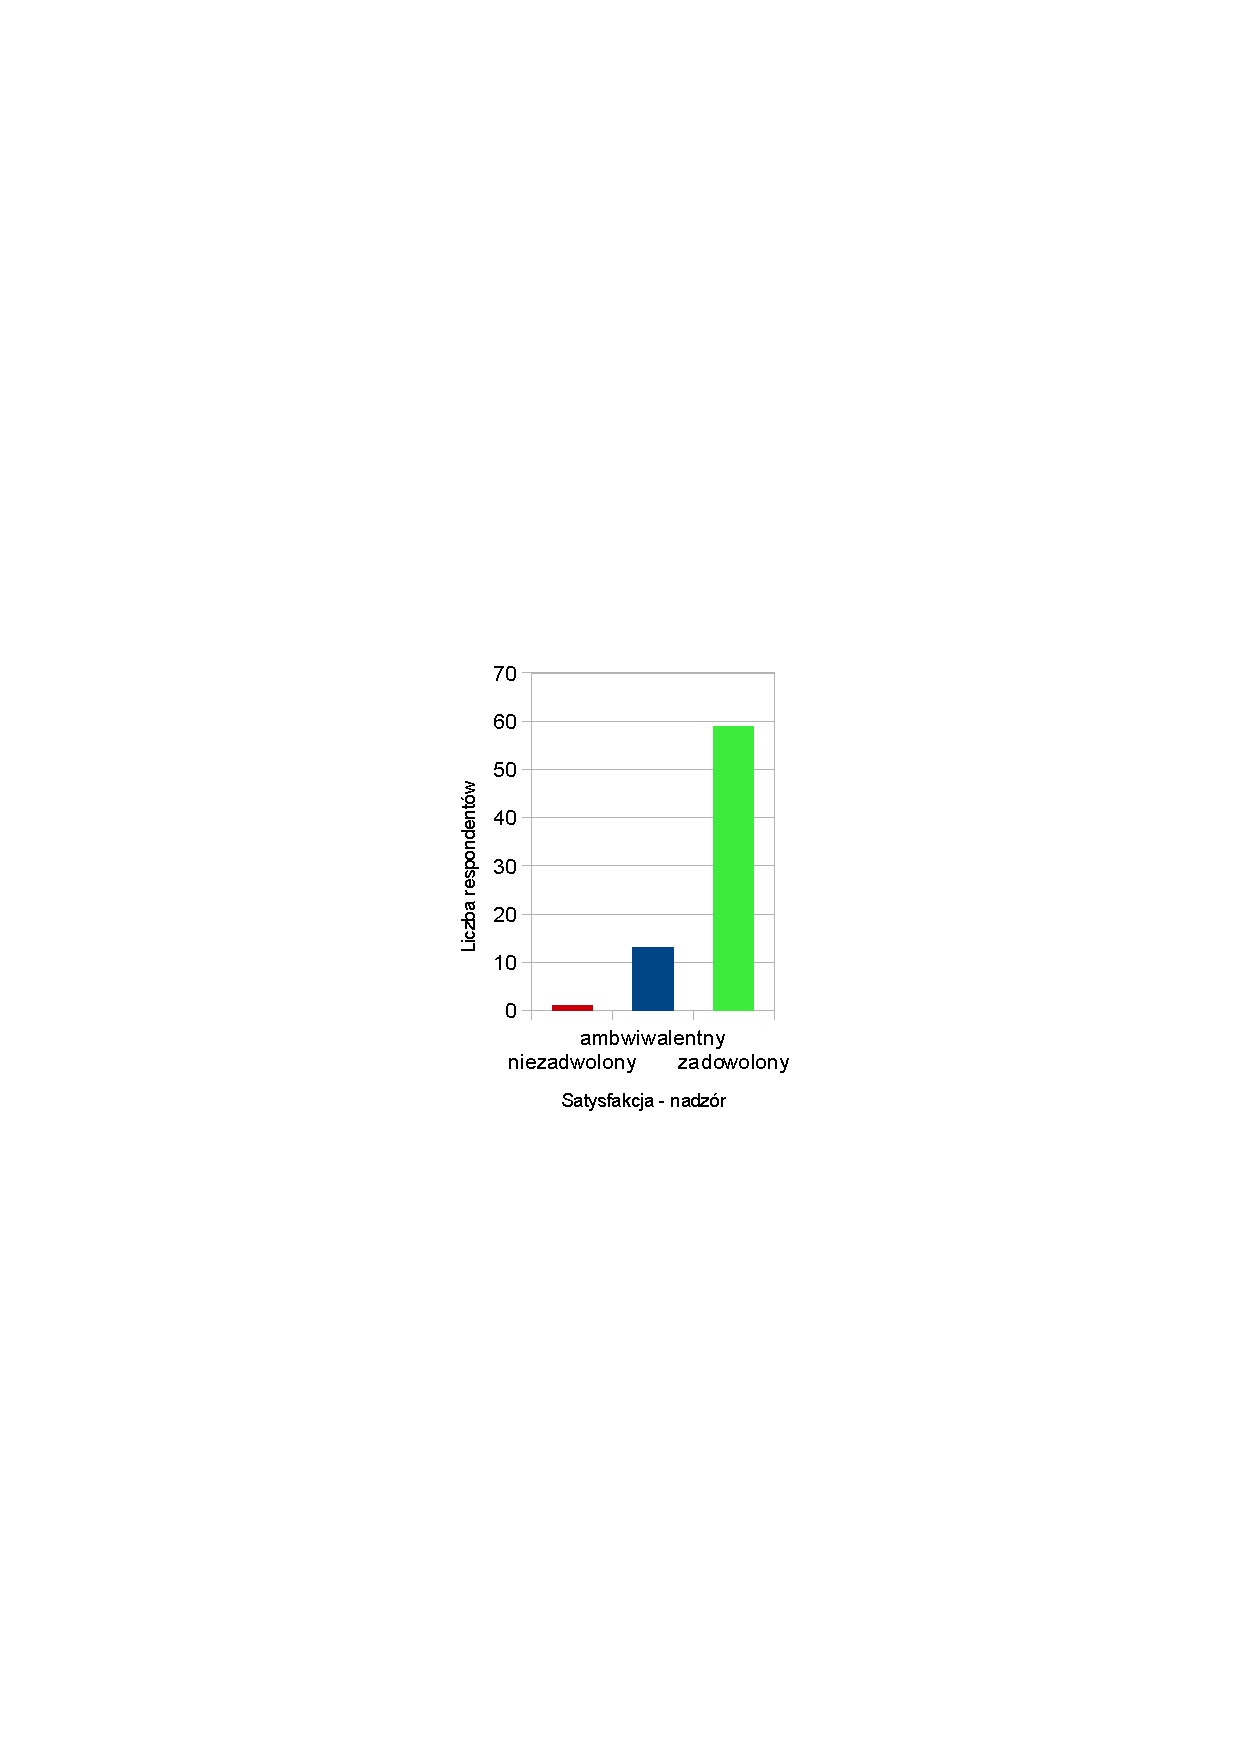
\includegraphics[height=0.27\textheight]{sat-supervision}}
    \subfloat[Dodatki]{\label{fig:his-benefits}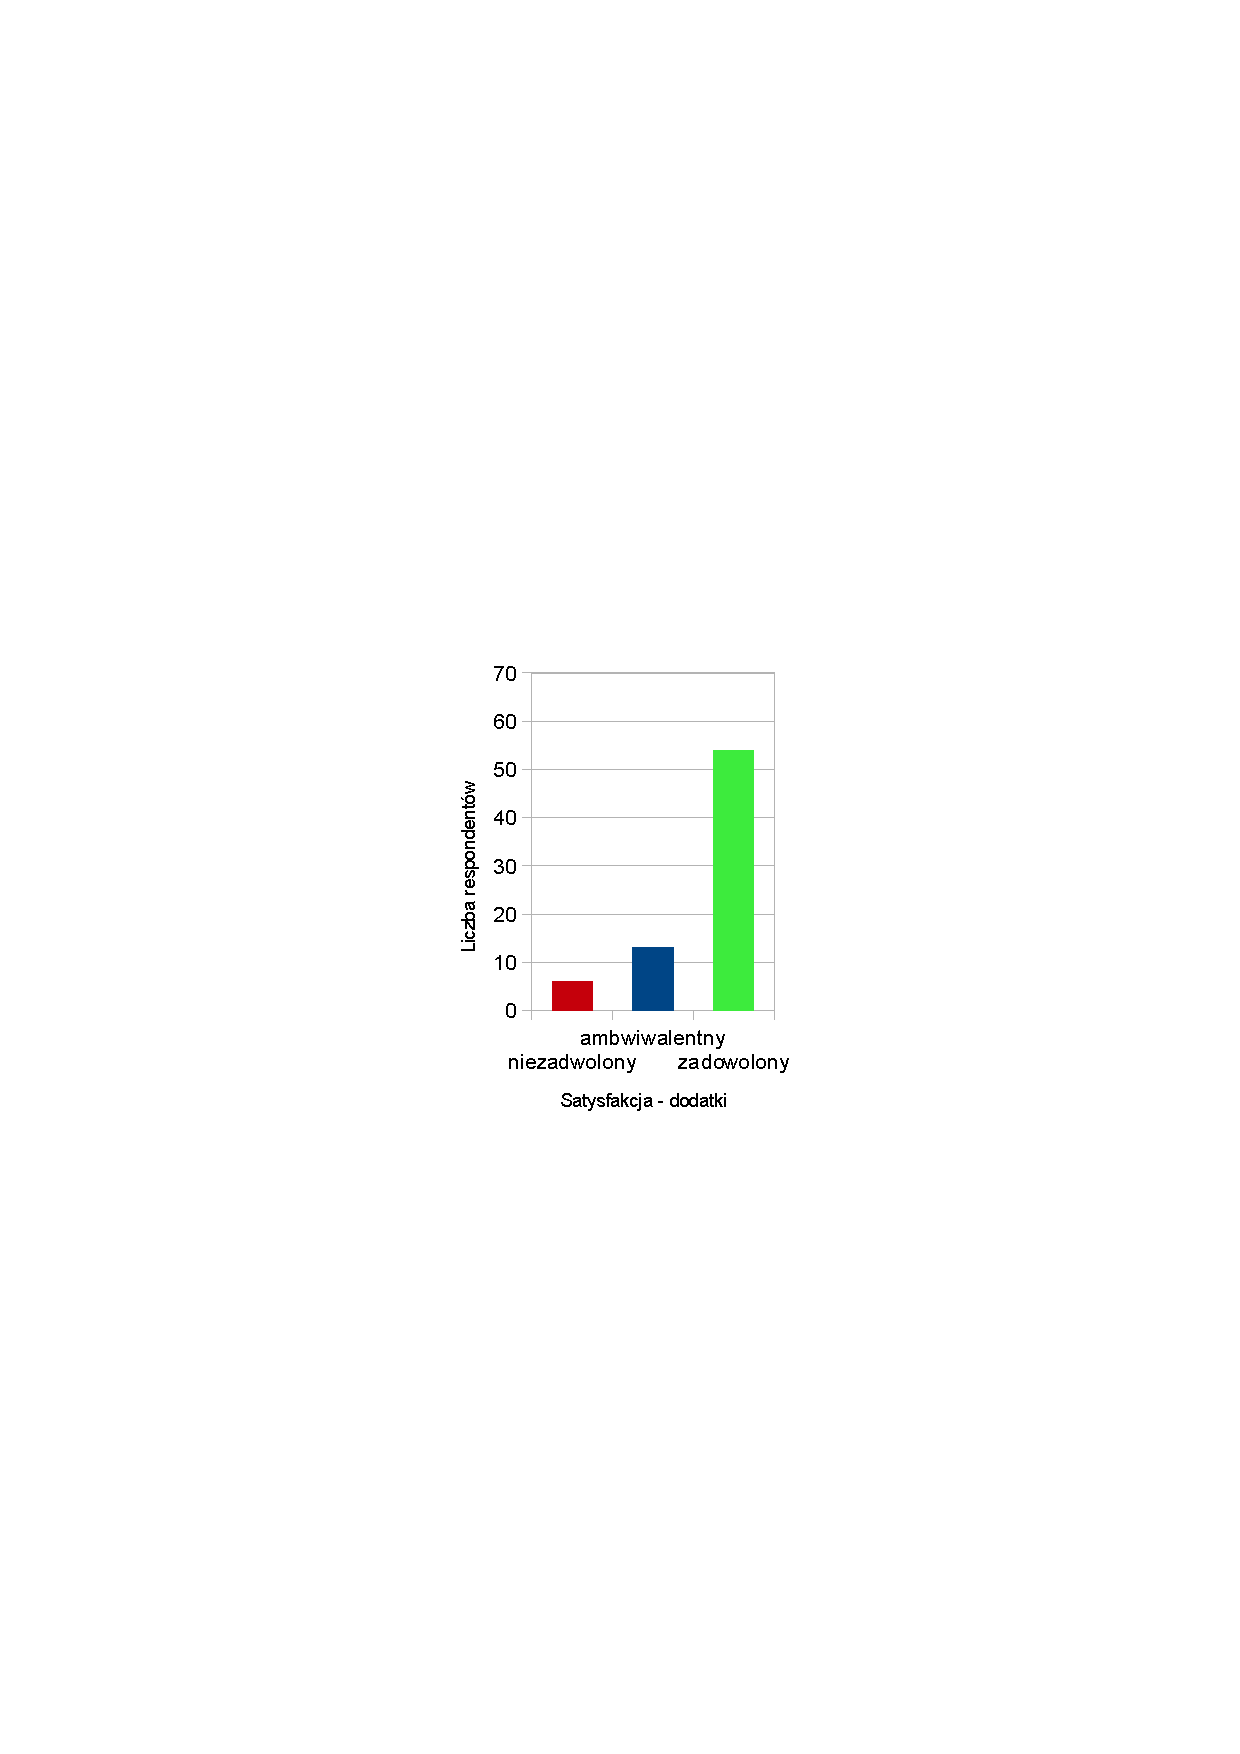
\includegraphics[height=0.27\textheight]{sat-benefits}}
    \\
    \subfloat[Nagrody]{\label{fig:his-rewards}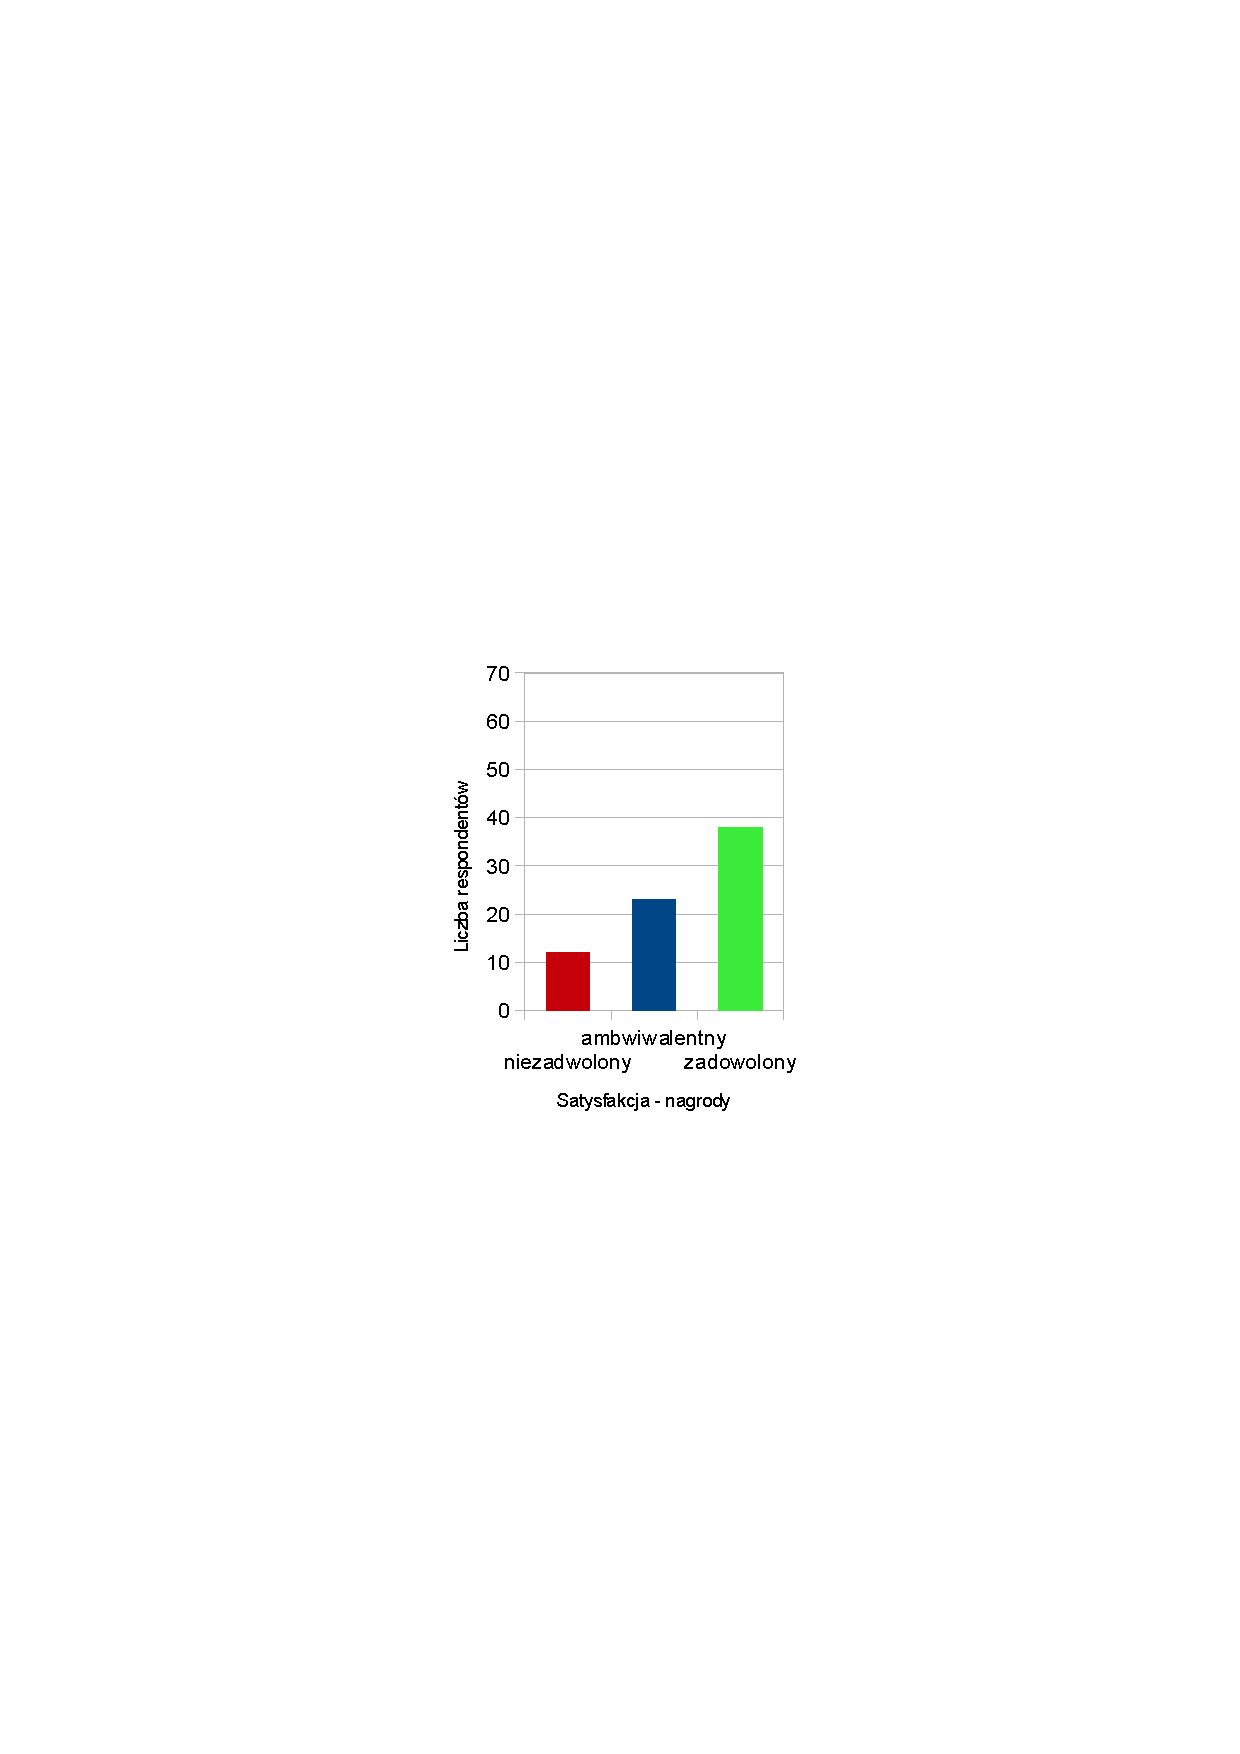
\includegraphics[height=0.27\textheight]{sat-rewards}}
    \subfloat[Warunki]{\label{fig:his-conditions}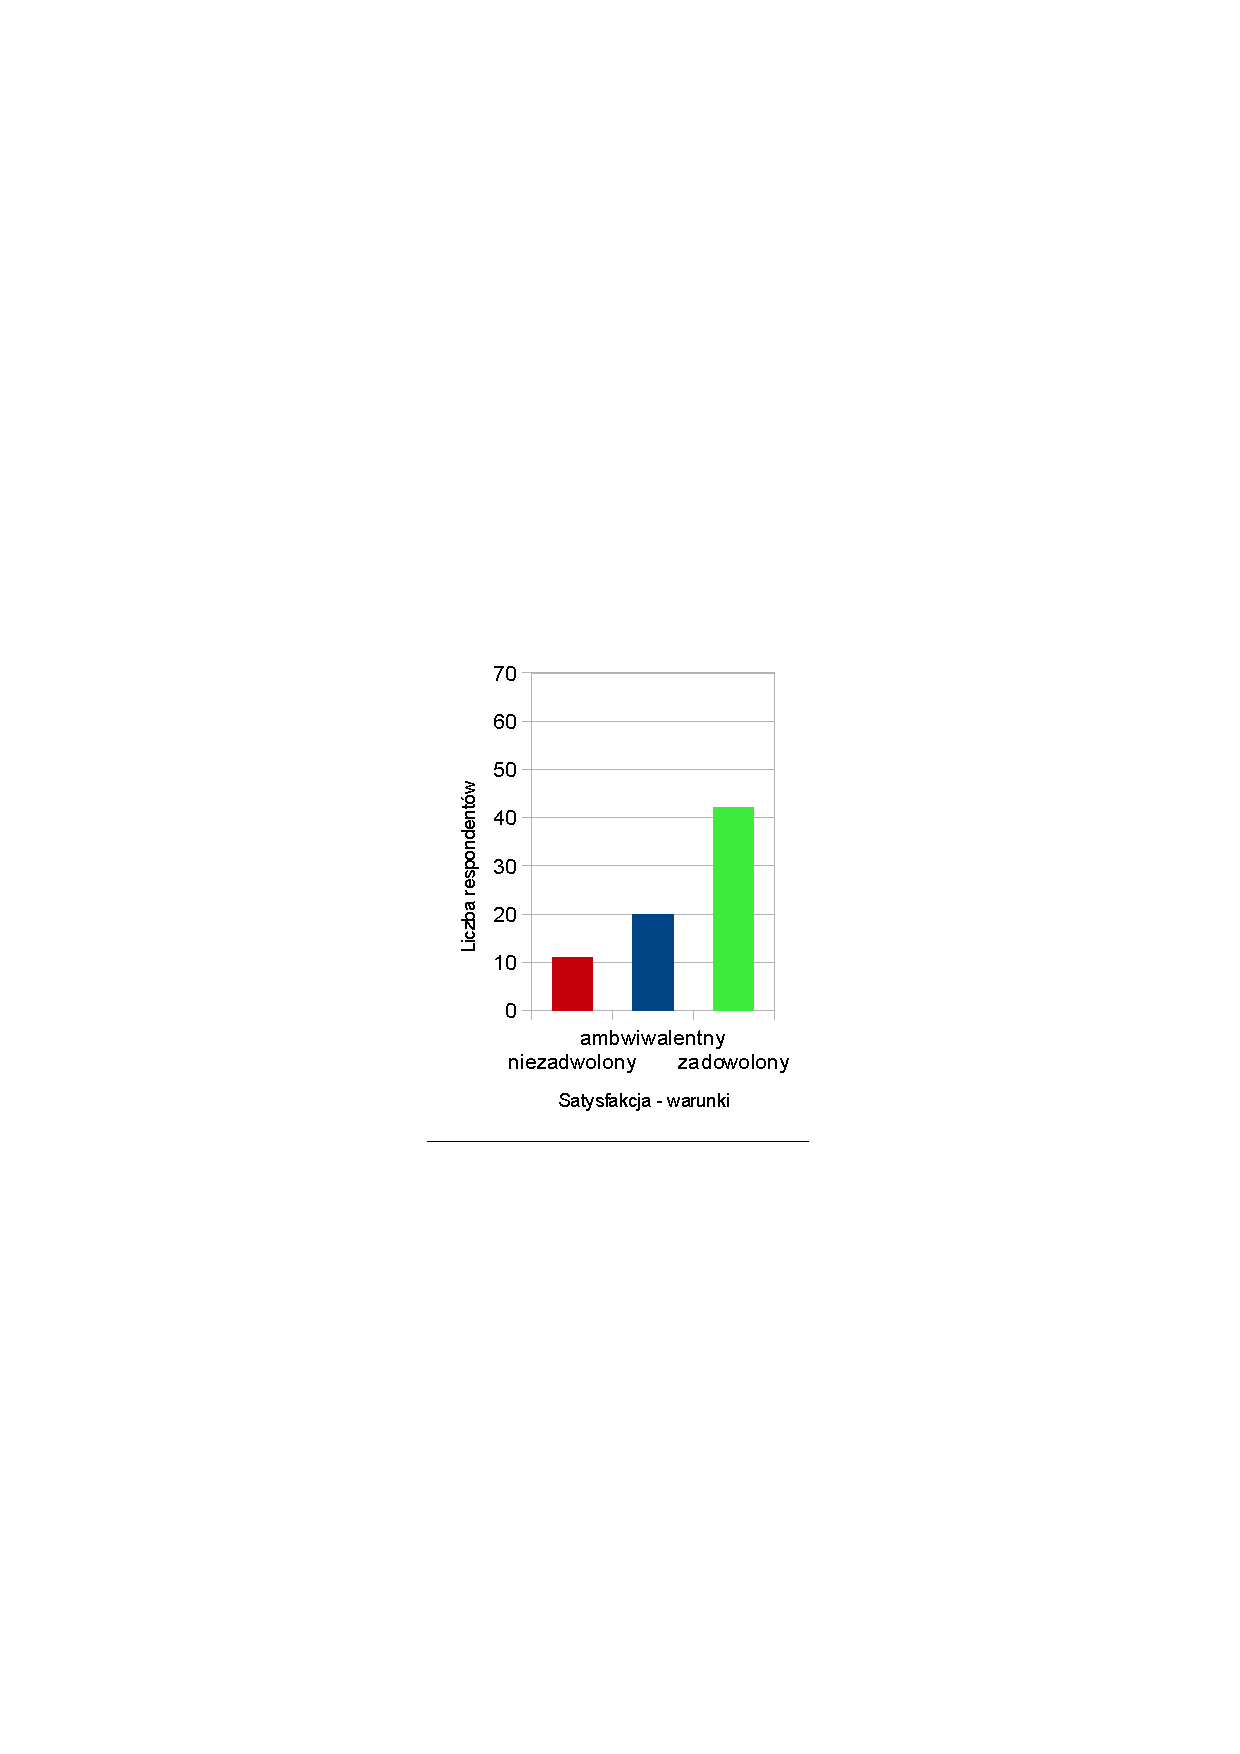
\includegraphics[height=0.27\textheight]{sat-conditions}}
    \caption{Histogramy dla \emph{JSS} -- część pierwsza}
\end{figure}

\begin{figure}[h!t]
    \centering
    \subfloat[Współpracownicy]{\label{fig:his-pay}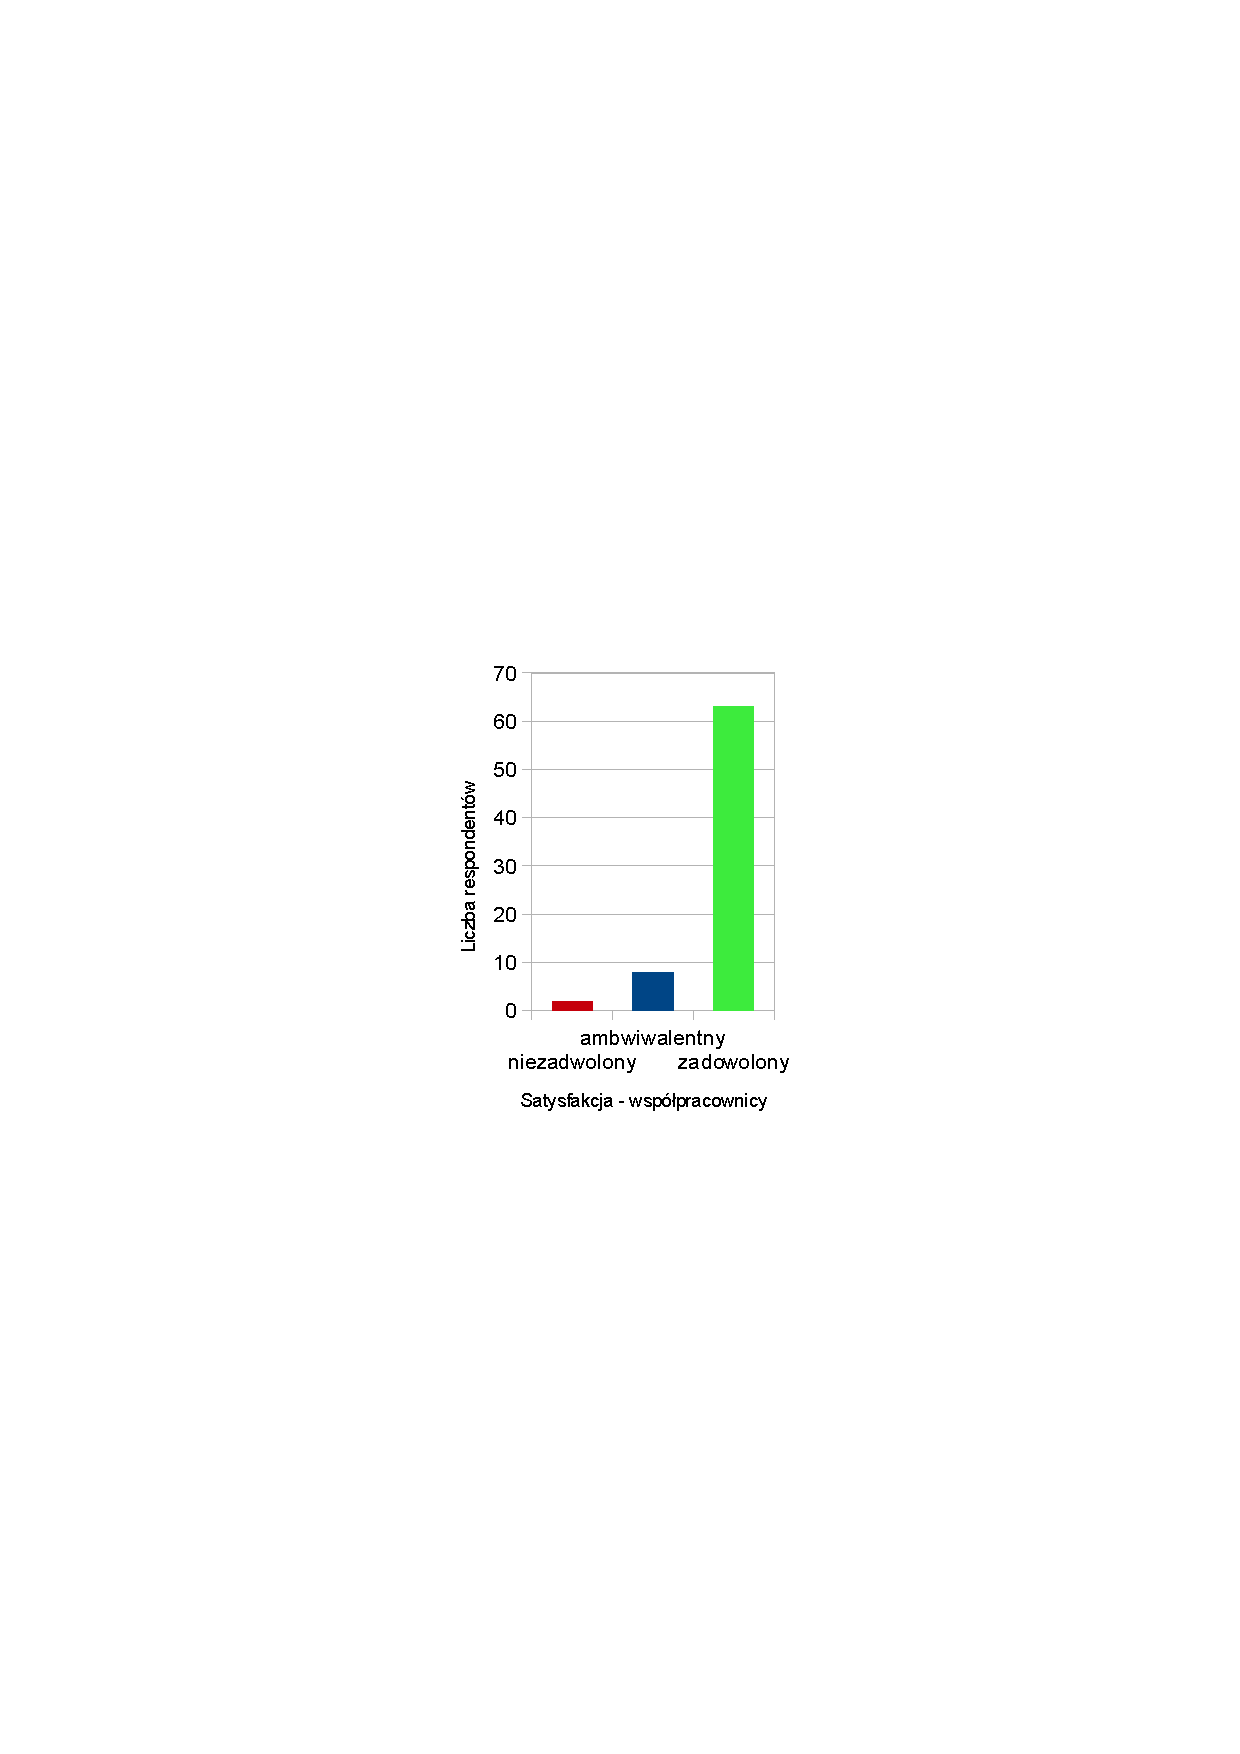
\includegraphics[height=0.27\textheight]{sat-coworkers}}
   \subfloat[Wykonywana praca]{\label{fig:his-promotion}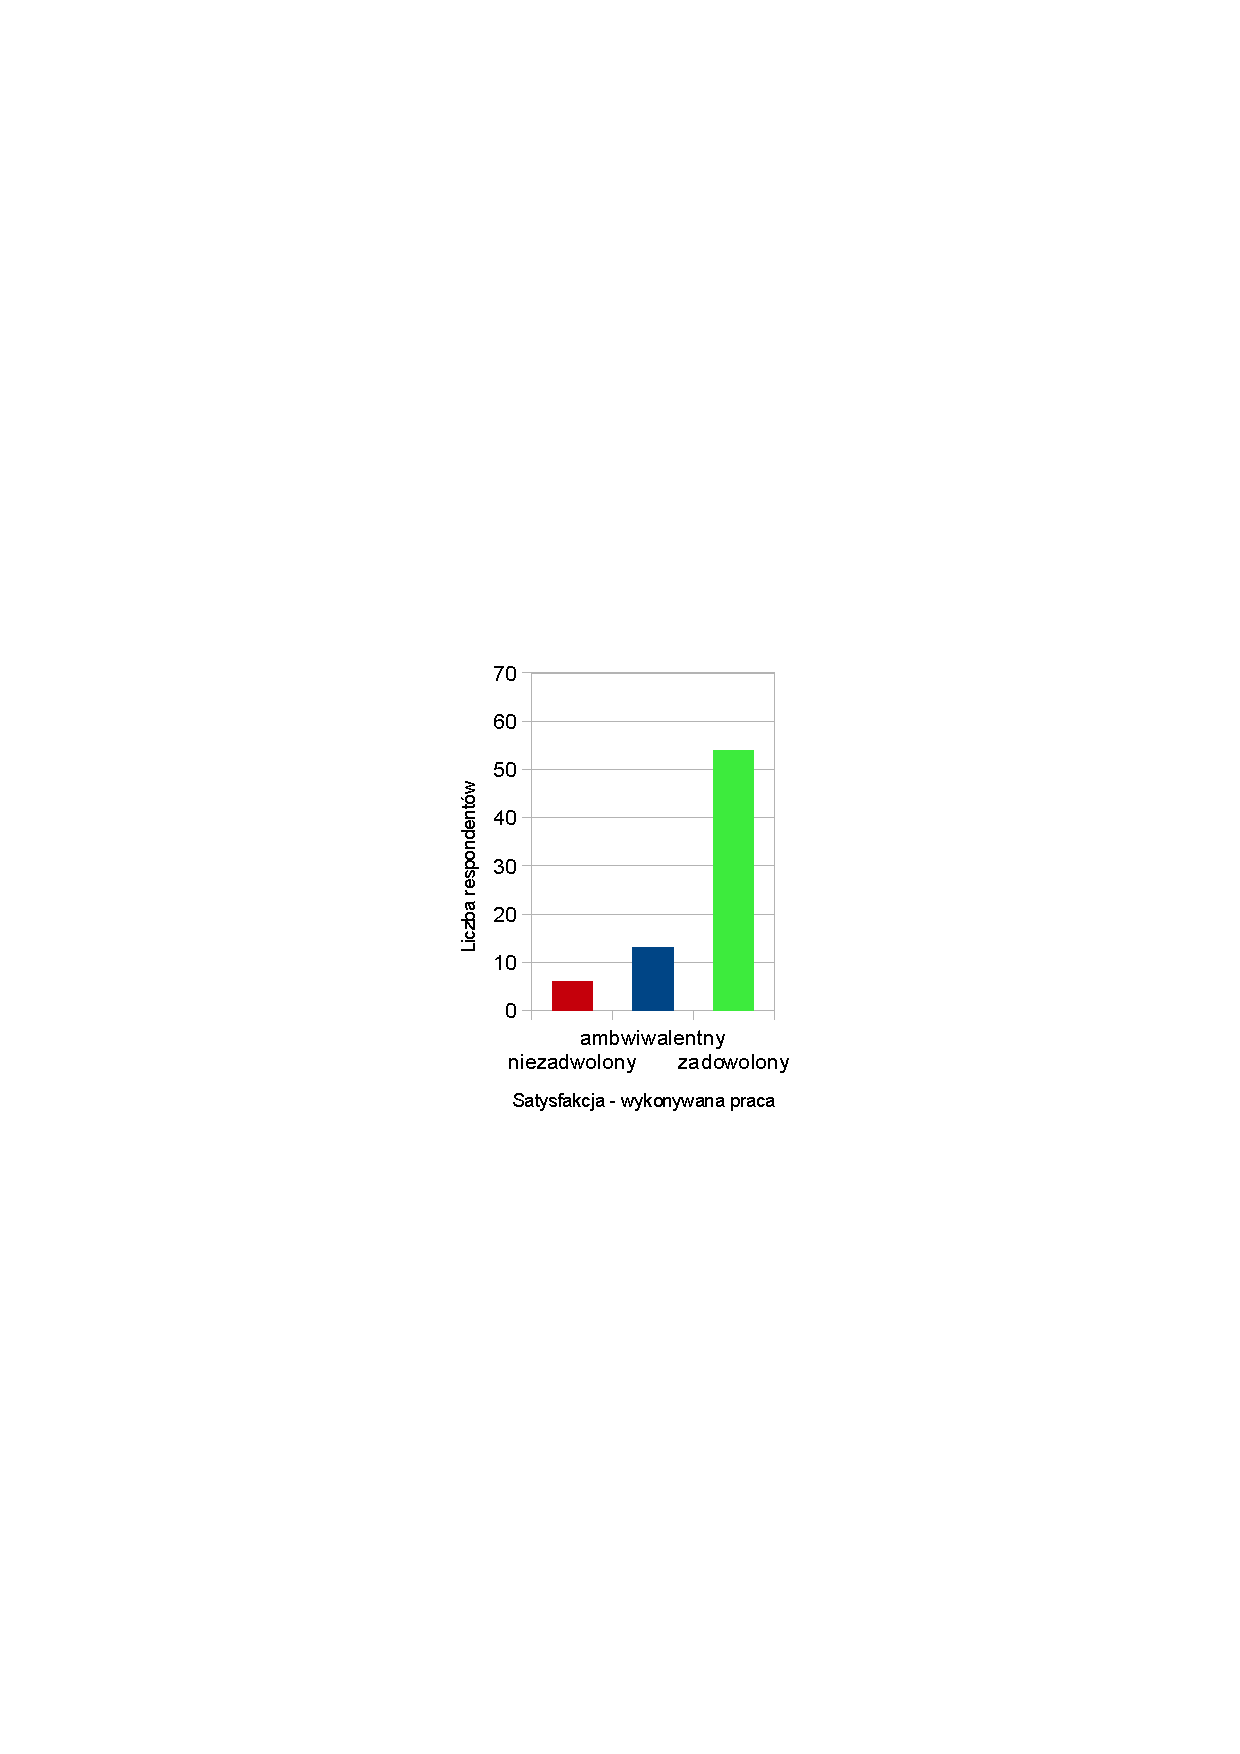
\includegraphics[height=0.27\textheight]{sat-work}}
    \\
    \subfloat[Komunikacja]{\label{fig:his-pay}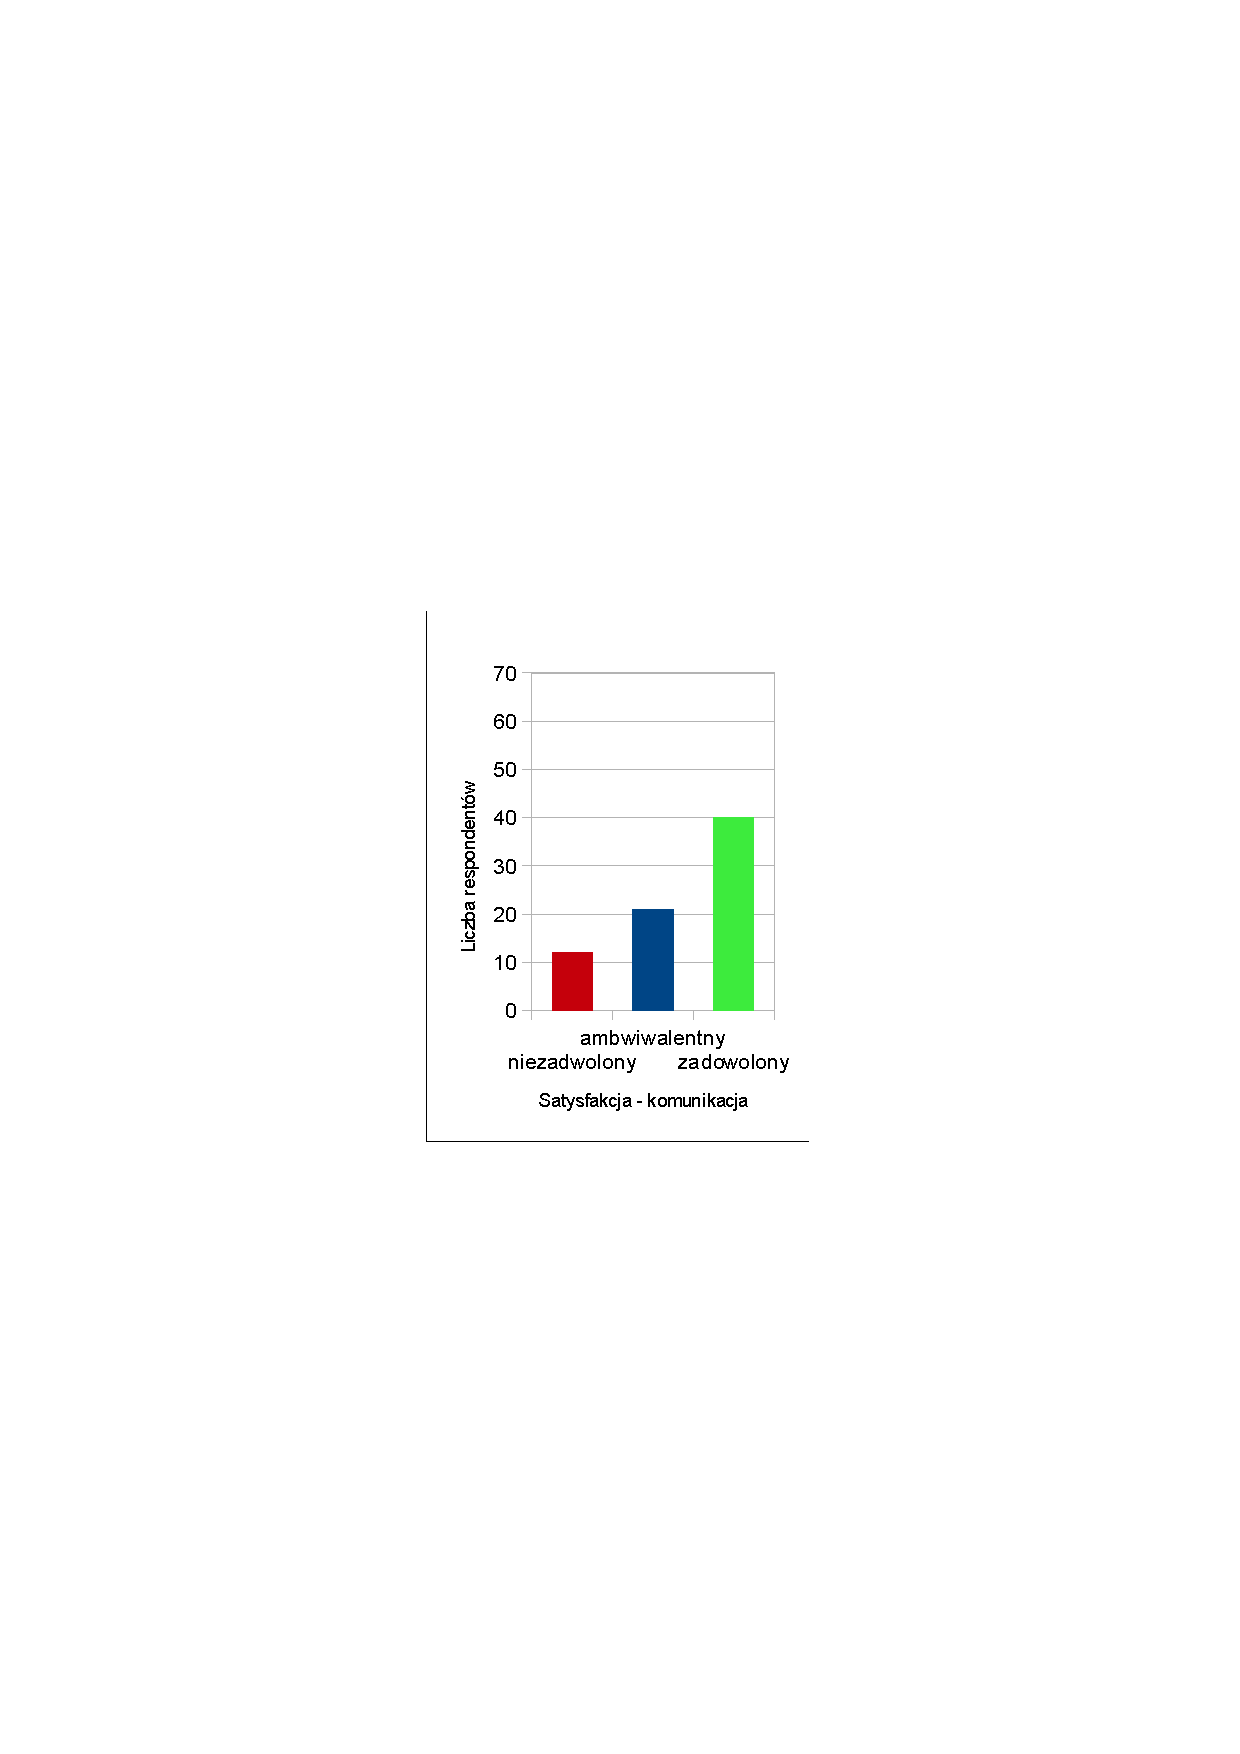
\includegraphics[height=0.27\textheight]{sat-communication}}
    \subfloat[Satysfkacja]{\label{fig:his-promotion}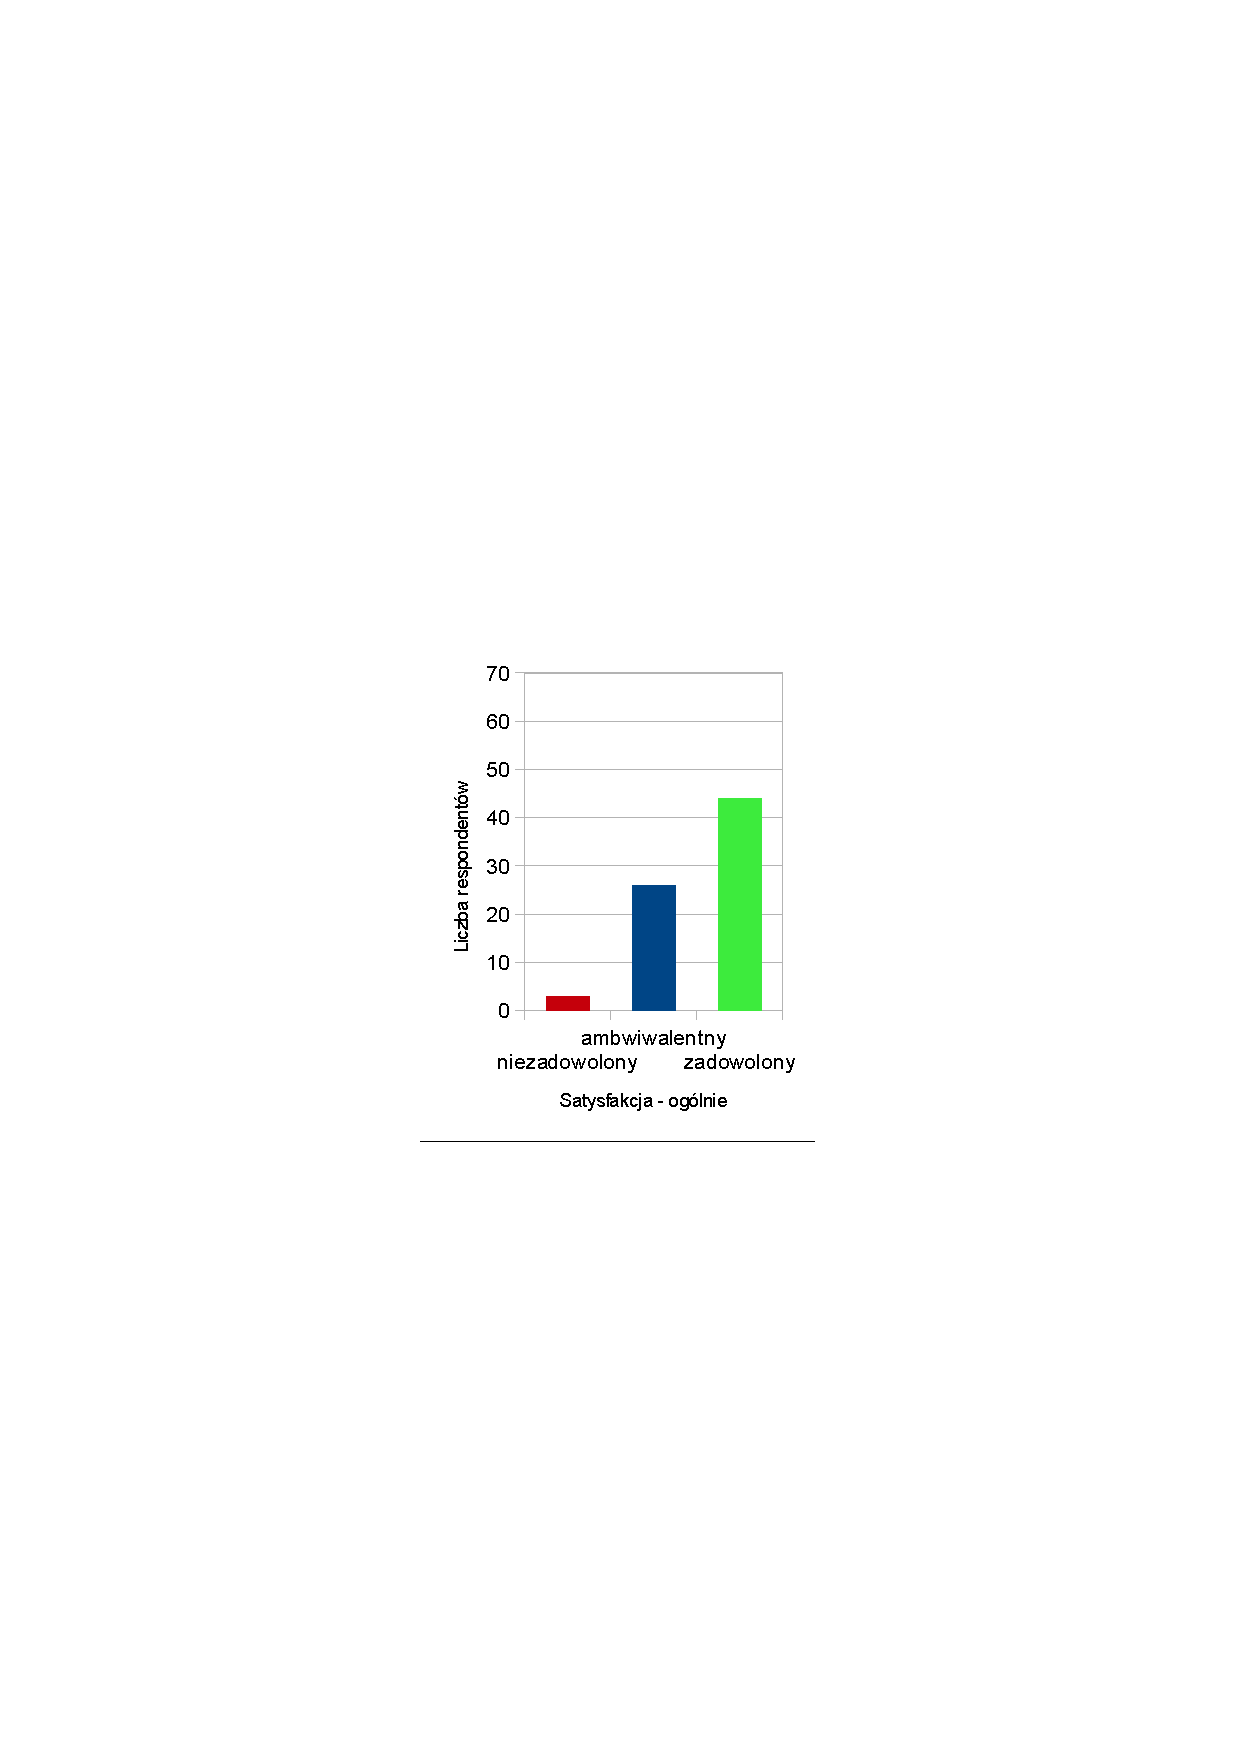
\includegraphics[height=0.27\textheight]{sat}}
    \caption{Histogramy dla \emph{JSS} -- część druga}
\end{figure}

\begin{table}[h!]
\begin{center}
\begin{tabular}{l | c c c c c c c c c c}
Wymiar & Min. & 1 kwartyl & Mediana & 3 kwartyl & Max.\\ \hline \hline
Płaca & 5 & 13 & 16 & 19 & 23 \\ 
Awanse & 4 & 10 & 14 & 17 & 23 \\
Nadzór & 10 & 17 & 20 & 22 & 24 \\
Dodatki & 9 & 15 & 18 & 20 & 24 \\
Nagrody & 5 & 13 & 16 & 19 & 24 \\
Warunki & 5 & 12 & 16 & 18 & 24 \\
Współpracownicy & 10 & 17 & 20 & 21 & 24 \\
Wykonywana praca & 6 & 15 & 19 & 21 & 24 \\
Komunikacja & 6 & 12 & 16 & 19 & 24 \\ \hline
Satysfakcja & 98 & 126 & 154 & 170 & 202 \\ \hline
\end{tabular}
\end{center}
\caption{Statystyki \emph{JSS} -- część pierwsza.}
\label{tab:jss-stats-1}
\end{table}

\begin{table}[h!]
\begin{center}
\begin{tabular}{l | c c c c c c c c c c}
Wymiar & Średnia & Moda & Wariancja & Odch. std. & Alfa Cronbacha\\ \hline \hline
Płaca & 15,99 & 19 & 18,57 & 4,31 & 0,77 \\
Awanse & 13,47 & 11 & 25,61 & 5,06 & 0,84 \\
Nadzór & 19,18 & 23 & 13,98 & 3,74 & 0,68 \\
Dodatki & 17,19 & 16 & 13,02 & 3,61 & 0,54 \\
Nagrody & 15,86 & 19 & 20,68 & 4,55 & 0,76 \\
Warunki & 15,51 & 16 & 17,5 & 4,18 & 0,59 \\
Współpracownicy & 19,08 & 20 & 9,35 & 3,06 & 0,58 \\
Wykonywana praca & 17,75 & 19 & 17,77 & 4,22 & 0,82 \\
Komunikacja & 15,62 & 12 & 18,27 & 4,27 & 0,67 \\ \hline
Satysfakcja & 149,64 & 125 & 645,51 & 25,41 & 0,91 \\ \hline
\end{tabular}
\end{center}
\caption{Statystyki \emph{JSS} -- część druga.}
\label{tab:jss-stats-2}
\end{table}

\begin{table}[h!]
\begin{center}
\begin{tabular} { l | c c c c c c c c c }
 & Pła & Awa & Nad & Dod & Nag & War & Wsp & Wp & Kom \\ \hline \hline
Pła & --- & 0,44 & 0,42 & 0,62 & 0,64 & 0,33 & 0,25 & 0,45 & 0,3 \\
Awa & & --- & 0,28 & 0,46 & 0,54 & 0,33 & 0,22 & 0,38 & 0,45 \\
Nad & & & --- & 0,49 & 0,58 & 0,28 & 0,41 & 0,47 & 0,38 \\
Dod & & & & --- & 0,66 & 0,38 & 0,34 & 0,46 & 0,32 \\
Nag & & & & & --- & 0,43 & 0,49 & 0,49 & 0,44 \\
War & & & & & & --- & 0,12 & -0,01 & 0,43 \\
Wsp & & & & & & & --- & 0,43 & 0,32 \\
Wp & & & & & & & & --- & 0,37 \\
Kom & & & & & & & & & ---  \\
\end{tabular}
\end{center}
\caption[Korelacja dla wszystkich wymiarów \emph{JSS}]{Korelacja dla wszystkich wymiarów \emph{JSS} (Pła -- Płaca, Awa -- Awanse, Nad -- Nadzór, Dod -- Dodatki, Nag -- Nagrody, War -- Warunki, Wsp -- Współpracownicy, Wp -- Wykonywana praca, Kom -- Komunikacja)}
\label{tab:jss-correl}
\end{table}

\paragraph{Płaca.} Na podstawie tabel \ref{tab:jss-stats-1} oraz \ref{tab:jss-stats-2} można ocenić, że wyniki rozpościerają się od 5 do 23, czyli pokrywają prawie całą skalę wartośći (oprócz wartości granicznych skali). Co ciekawe, mediana (wartość 16) oraz wartość średnia (15,99) znajduje się dokładnie na granicy między ambwiwalentnym stosunkiem do płacy, a zadowoleniem. W związku z tym można stwierdzić, że ok. połowa pracowników sektora IT jest zadowolona ze swojej pracy. Odchylenie standardowe 4,31 na pięciostopniowej skali nie jest ani duże ani małe. Wskazuje
jednak na średnie wachania w danych. Z zadowalających rzeczy, alfa Cronbacha jest powyżej 0,7 (dokładnie 0,77) co wskazuję na spójność odpowiedzi w ramach wymiaru.

Patrząc na Tabelę \ref{tab:jss-correl} \textit{płaca} ma wysoki współczynnik korelacji z ogólną satysfakcją (dokładnie 0,73). Co było do przewidzenia, najniższa korelacja istnieje dla czynników pozafinansowych, społecznych: \emph{współpracowników} oraz \emph{komunikacji}

\paragraph{Awans.} Podobnie jak z \textit{płacą}, wyniki dla \emph{awansu} rozpościerają się prawie na całej skali (oprócz wartości maksymalnej dla skali). Pierwszy kwartyl i mediana znajduą się na poziomie niezadowolenia i niepewnego stosunku do tego aspektu pracy. Trzeci kwartyl (wartość 17) jest tylko nieznacznie w przedziale zadowolenia. Widać to wyrażnie na histogramie \emph{awansu} (Rysunek \ref{fig:his-promotion}) -- ponad połowa osób nie jest zadowolona
z możliwości awansu w pracy. Dodatkowo odchylenie standardowe jest duże -- 5,06 i wskazuje na duży rozrzut w danych. Przy czym jest to wymiar satysfakcji, który jest najbardziej spójny jeżeli chodzi o odpowiedzni na zadane pytania. Uzyskał wynik 0,84 dla alfy Cronbacha.

Analizując Tabelę \ref{tab:jss-correl} widzimy, że najwyższa korelacja tego aspektu pracy jest z \textit{nagrodami}. Jednak jest to wartość nieznacznie powyżej 0,5 (dokładnie 0,54). W następnej kolejności są \emph{dodatki}. Jest to zgodne z formą przyznawania awansów i nagród, są to formy uznania przez przełożonego i podlegją jego subiektywnej ocenie. Co ciekawe, z drugiej strony, korelacja z wymiarem oceny przełożonego (\emph{nadzór}) jest słaba. Wskazuje to na niesymetryczność w
ocenie na poziomie relacji szef-przełożony. Uzupełniając, z resztą wymiarów \textit{awans} jest słabo skorelowany. 

Ogólnie wyniki dla \textit{awansu} są najsłabsze w porównianiu z innymi wymiarami. Oznacza to, że jest to aspekt pracy, z której pracownicy są najmniej zadowoleni.

\paragraph{Nadzór.} Skala dla \textit{nadzoru} zaczyna się dopiero od wartości 10 i kończy na maksmalnej możliwej -- 24. Pierwszy kwartyl (wartość 17) znajduje się na poziomie satysfakcji z pracy, mediana to 20, a trzeci kwartyl to 22 (tylko dwa punkty przed końcem skali). Jeżeli dodamy do tego średnią na pizomie 19,18 oraz modę równą 23 widać wyraźnie, że większość respondentów jest bardzo zadowolonych ze swoich przełożonych. Widać to bardzo dobrze na histogramie na Rysunku
\ref{fig:his-supervision}. Dodatkowo w miarę niskie odchylenie standardowe
na poziomie 3,74 wskazuje na mały rozrzut wartości w danych. Co ciekawe alfa Cronbacha jest na granicy akceptowalności (TODO kto to wyznaczył -> znajdź w UWES)a i wynosi 0,68.

Natomiast w Tabeli \ref{tab:jss-correl} znajdują się korelacje między \textit{nadzorem}, a innymi wymiarami \textit{satysfakcji}. Najwyższa wartość jest powiązana z otrzymywanymi nagrodami (wymiar \textit{nagrody}) i wynosi 0,58 (czyli nieznacznie ponad 0,5 -- średniej siły korelacja). Oznacza to, że przełożonych doceniamy najbardziej za nagrody jakie od nich otrzymujemy, czyli dodatkowe formy uznania naszej pracy. Następnie w kolejności są \textit{dodatki} (0,49), a
później \textit(wykonywana praca) (0,47). Interesująca jest zależność z wykonywaną pracą, wskazuje to na docenienie szefa za zlecane zadania. Z drugiej strony, niska korelacja z wymiarem \textit{warunków} oraz \textit{komunikacji} wskazuje na oczekiwania jakie pracownicy stawiają swoim przełożonym. O dziwio nie wiążą się one z ułatwianiem pracy (np: warunki, które sprzyjają wydajnej pracy, jasno stawiane cele), chociaż takie teoretycznie powinny być m.in. wymagania wobec przełożonych.

\paragraph{Dodatki.}\label{par:res-benefits} Przyjmowane wartości przez ten wymiar zaczynają się dopiero od 9 i ciągną się do maksymalnej wartości. Pierwszy kwartyl jest blisko granicy między abwiwalentnymi odczuciami, a satysfakcją. Czyli ok. 75\% respondentów jest zadowolona ze swoich dodatków. Mediana (wartość 18), trzeci kwartyl (wartość 20) i średnia (wartość 3,61) znajdują się już w granicach pułapu dla określenia satysfakcji. Widać to bardzo ładnie na histogramie wartości na
Rysunku \ref{fig:his-benefits}. Jeżeli dodamy do tego dość niskie
odchylenie standardowe o wartości 3,61 widzimy, że respondenci są całkiem zgodni jeżeli chodzi o zadowolenie z otrzymywanych dodatków. Z drugiej strony Alfa Cronbacha jest najniższa ze wszystkich wymiarów i wynosi 0,54. Wskazuje to na najmniejszą spójność w odpowiedziach na pytania odnośnie dodatków w pracy.

Przyglądając się korelacji w Tabeli \ref{tab:jss-correl}, najwyższą wartość posiada z \textit{nagrodami} (wartość 0,66) oraz z \textit{płacą} (wartość 0,62). Jest to zgodne z założeniami, że jeżeli firmę stać na dodatki takie jak dodatkowy pakiet medyczny dla pracowników, posiada ona wysokie zasoby pienieżne, tak aby móc wypłacać wysokie pensje. Przyczyna ta może, ale nie musi, wiązać się z wypłacaniem nagród czy też ich rodzajem. 

\paragraph{Nagrody.} \textit{Nagrody} mają bardzo podobne statystyki co \textit{płace}. Minimalna wartość to 5, pierwszy kwartyl to 13, mediana (wartość 16) jest na granicy między ambwiwalentnym stosunkiem, a satysfakcją. Trzeci kwartyl to 19. Tylko wartość maksymalna jest o 1 większa i wynosi 24. Jeżeli dodamy do tego średnią na poziomie 15,86 (czyli granica między ambwiwalencją, a satysfakcją) i spojrzymy na histogram wartośći na Rysunku \ref{fig:his-rewards},
dostrzegamy, że ok. połowa badanych jest zadowolona z orzymywanych nagród, jedna-trzecia ma odczucia mieszane, reszta jest po prostu niezadowolona. Dodatkowo odchylenie standardowe jest na średnim poziomie i wynosi 4,55. Wskazuje to na średni rozrzut danych w odpowiedziach badanych. Za to alfa Cronbacha jest bardzo wysoka i wynosi 0,76 (powyżej granicy 0,7) i wskazuje na rzetelność tej skali.

Patrząc na Rysunek \ref{tab:jss-correl} widzimy korelacje dla \textit{nagród}. Najzwyższa jest z \textit{dodatkami} oraz z \textit{płacą}. Możliwe przyczyny zostały już opisywane w paragrafie wyżej nt \textbf{dodatków} (sekcja \ref{par:res-benefits}). Wysoka korelacja jest także z \textit{awansami} (wartość 0,54) oraz \textit{nadzorem} (wartość 0,58). \textit{Awanse} mogą się wiązać z podobieństwiem przyczyny otrzymywania \textit{nagród} i \textit{awansów} -- jest to forma
docenienia dobrej pracy pracownika. Czyli pracownicy, którzy dostają dużo nagród są brani pod uwagę przy awansach i prawdopodobnie szybciej pną się po szczeblach kariery. Natomiast co do \textit{nadzoru} wydaje się to być naturalnym, że mamy pozytywny stosunek do osób, które w jakiś sposób nas doceniają.

\paragraph{Warunki.} Skala dla warunków rozciąga się od prawie minimalnej wartości (5) do maksymalnej możliwej (24). Pierwszy kwartyl (wartość 12) znajduje się na granicy niezadowolenia i niepewnych odczuć, co oznacza, że mniej niż 25\% pracowników nie odczuwa satysfakcji z pracy. Mediana (wartość 16) jest na granicy między mieszanymi odczuciami, a zadowoleniem z pracy (podobnie jak średnia -- 15,51) -- co oznacza razem z pierwszy kwartylem ponad 25\% ambwiwalentnych. Trzeci kwartyl (wartość 18) to już zadowlenie, czyli ok. 50\% jest zadowolonych ze swoich
warunków z pracy. Potwierdza to wykres histogramu na Rysunku \ref{fig:his-conditions}. Wariancja jest średnio wysoka i wynosi 4,18. Wskazuje to na w miarę duże różnice w odpowiedziach respondentów. Natomiast co do rzetelności skali, to alfa Cronbacha jest powyżej progu 0,7 i wynosi 0,76 co wskazuje na spójne odpowiadanie na zadane pytania.

Przechodząc do korelacji, \textit{warunki} posiadają najwyższą wartość dla tego współczynnika dla \textit{komunikacji} i \textit{nagród} -- oba wynoszą 0,43 (średnia korelacja). Jeżeli chodzi o \textit{nagrody} można to wytłumaczyć tym, że jeżeli firmę stać na pokrywanie zadowalających nagród dla pracowników, wówczas stać ich także na zapewnienie zadowalających warunków pracy. Za to ciekawa jest korelacja z \textit{komunikacją}. Możliwe, że jeżeli komunikacja w ramach firmy jest dobra, to informacje o niedociągnięciach w
środowisku pracy docierają do odopowiednich osób i dzięki temu warunki się poprawiają. 

\paragraph{Współpracownicy.} Minimalna wartość dla \textit{współpracowników} zaczyna się dopiero od 10 i rozciąga się do maksymalnej możliwej wartości. Pierwszy kwartyl to 17 (czyli już na poziomie zadowolenia z pracy), mediana to 20, a trzeci kwartyl to 21. Jeżeli dodamy do tego średnią na poziomie 19,08 oraz odchylenie standardowe najniższe ze wszystkich - 3,06, widzimy, że respondenci byli zgodni co do wysokiej opini na temat swoich współpracowników. Potwierdza to wykres
na Rysunku \ref{fig:his-coworkers}. Co ciekawe metryki te są bardzo podobne jak dla \textit{pracy}. Dodatkowo alfa Cronabach jest jedną z najniższych i wynosi 0,58. Wskazuje to na możliwą niespójność w odpowiedziach badanych między konkretnymi pytaniamia w ramach wymiaru.

Przechodząc do korelacji (patrz Tabela \ref{tab:jss-correl} widzimy, że najwyższa wartość jest dla \textit{nagród} (wartość 0,49), a następnie dla \textit{wykonywanej pracy} (wartość 0,43). Relacja o średniej sile z \textit{nagrodami} początkowa wydaje się zaskakujące. Możliwe, że przyczyną są warunki finansowe firmy, tzn. jeżeli organizację stać na przekazywanie pracownikom zadowalających nagród, to także stać ich na zatrudnianie bardzo dobrych pracowników z dostępnych
na rynku pracy. Natomiast zależność z \textit{wykonywaną pracą} może wiązać się z profesjonalizmem współpracowników. Ludzie lubią prace, które są dla nich łatwe do zrozumienia (dopasowane do ich umiejętności, tzw. odpowiedniość pracy). Dzięki swojemu wysokiemu poziomowi wiedzy są w stanie wesprzeć innych pracowników podczas pracy.

Warto podkreślić, że jest to wymiar, z którego najwięcej osób jest zadowolonych (ok. 90\% respondentów).

\paragraph{Wykonywana praca.} Wyniki dla tego wymiaru rozpościerają się prawie na całej skali oprócz pierwszych dwóch najniższych wartośći. Pierwszy kwartyl (wartość 15) znajduje się na poziomie mieszanych uczuć, co oznacza, że co najmniej 25\% osób jest niezadowolonych lub nie jest pewnych swoich odczuć do wykonywanych zadań. Mediana (wartość 19) znajduje się już na poziomie zadowolenia, tak samo jak trzeci kwartyl (wartość 21). Czyli co najmniej 50\% respondentów jest zadowolonych z
natury ich pracy. Dane te potwierdza histogram na Rysunku \ref{fig:his-work}. Dodatkowo rozrzut odpowiedzi uczestników jest średniej wielkość (odchylenie standardowe to 4,22). Natomiast spójność skali jest bardzo wysoka (alfa Cronbacha 0,82).

Co do korelacji z Tabeli \ref{tab:jss-correl} \textit{wykonywana praca} najwyższą wartość ma dla \textit{nagród} (wartość 0,49), następnie \textit{nadzoru} (wartość 0,47) oraz \textit{dodatków} (wartość 0,46). \textit{Nagrody} oraz \textit{nadzór} można wiązać się z dobrym wykonywaniem zleconej pracy. Wiąże się to z otrzymywaniem nagród uznaniowych oraz chwaleniem przez przełożónych. Natomiast w wypadku \textit{dodatków} zależność może być w drugą stronę, tzn. miejsce pracy, które udostępnia swoich
pracowników dodatki (np.: karnet na siłownie) przyciąga bardziej zdolne osoby z rynku pracy, które lubią to co robią i robią to dobrze.

\paragraph{Komunikacja.} Wartości dla komunikacji rozciągają się od 6 do 24 (prawie cała skala). Pierwszy kwartyl (wartość 12) znajduje się na granicy między satysfakcją, a mieszanymi odczuciami. Mediana znajduje się na poziomie 16, czyli na granicy między ambwiwalencją, a zadowoleniem. Wynika z tego, że trochę mniej niż 25\% respondentów nie jest zadowolonych z tego aspektu swojej pracy i mniej więcej tyle samo ma ambwiwalentne uczucia. Trzeci kwartyl na poziomie 19 to
już zadowolenie z pracy. Czyli trochę ponad 50\% respondentów jest usatysfakcjonowanych komunikacją w miejscu pracy. Przyglądając się histogramowi z Rysunku \ref{fig:his-communication} widzimy, że osób niezadowolonych (12 osób, ok. jedna-szósta badanych) jednak jest o połowę mniej niż z mieszanymi odczuciami (21 osób, ok. jedna-trzecia badanych). Co ciekawe moda jest na wartośći 12, czyli granicznej między brakiem zadowolenia, a mieszanymi odczuciami. Jeżeli założymy, że 12 to jeszcze przedział
niezadowolenia wyniki wyglądają następująco: niezadowolenie -- 22 osoby, abwiwalencja -- 11 osóbk, czyli praktycznie na odwrót. W tym przypadku widzimy, jak delikatną sprawą jest określenie granic przedziałów i jak mogą one wpływać na końcową interpretację. Dlatego warto patrzeć na wszystkie miary statystyczne odnośnie danyhc (w tym przypadku medianę). 

Rozrzut odpowiedzi badanych był średnio wysoki, odchylenie standardowe wynosi 4,27. Natomiast alfa Cronbacha na poziomie 0,67 znajduje się na granicy 0,7 i można przyjąć, że skala ta jest skalą spójną (tzn. respondenci odpowiadali spójnie na pytania w ramach tej skali).

Patrząc dalej na Tabelę \ref{tab:jss-correl} z korelacjami, \textit{komunikacja} najwyższą zależność ma z \textit{awansami} (wartość 0,45), następnie istnieje zależność z \textit{nagrodami} (wartość 0,44). Jeżeli osoba jasno rozumie cele firmy, jest w stanie je realizować dobrze, a co za tym idzie spełniać oczekiwania i być promowanym oraz otrzymywać nagrody. Zbliżoną wartość mają także \textit{warunki} (wartość 0,43). Możliwe, że jasna komunikacja na linii
kierownictwo--przełożeni owocuje lepszym zrozumieniem potrzeb pracowników, a co za tym idzie także dostosowaniem warunków pracy do ich optymalnego wykonywania zadań.

\paragraph{Satysfakcja ogólna.}
Przymowane wartości rozciągają się od 98, do 202 (domena od 36 do 216). Dodając do tego pierwszy kwartyl (wartość 126) w granicach abwiwalentnych odczuć oraz medianę (wartość 154) oraz trzeci kwartyl (wartość 170), widzimy, że ponad 50\% respondentów jest zadowolonych ze swojej pracy. Średnia o wartośći 149,64 znajduje się także w przdziale zadowolenia. Dane te potwierdza histogram na Rysunku \ref{fig:his-sat}. Widzimy tam także, że osoby o mieszanych odczuciach to ok.
jedna-trzecia grupy, natomiast osoby niezadowolone całkowicie to znikoma ilość respondentów (dokładnie 3 osoby).

Odchylenie standardowe wynosi 25,41, czyli dla skali o szerorokości 180 jest to średnio-niski wynik, czyli średni rozrzut w danych. Natomiast alfa Cronbacha ma bardzo wysoki wynik i wynosi 0,91, co wskazuje na dużą spójność w odpowiedziach respondentów.

\FloatBarrier

\subsection{Ultrech Work Engagement Survey}

\begin{table}[h!]
\begin{center}
\begin{tabular}{l | c c c c c c c c c c}
Wymiar & Min. & 1 kwartyl & Mediana & 3 kwartyl & Max.\\ \hline \hline
Wigor & 1,33 & 3 & 3,83 & 4,67 & 5,5 \\
Oddanie & 1,4 & 3 & 4 & 4,8 & 6 \\
Absorpcja & 1,17 & 3 & 3,5 & 4,67 & 5,83 \\ \hline
Zaangażowanie & 1,47 & 3 & 3,5 & 4,53 & 5,59 \\
\end{tabular}
\end{center}
\caption{Statystyki \emph{UWES} -- część pierwsza.}
\label{tab:uwes-stats-1}
\end{table}

\begin{table}[h!]
\begin{center}
\begin{tabular}{l | c c c c c c c c c c}
Wymiar & Średnia & Moda & Wariancja & Odch. std. & Alfa Cronbacha\\ \hline \hline
Wigor & 3,75 & 4 & 1,13 & 1,06 & 0,83 \\
Oddanie & 3,79 & 4,2 & 1,47 & 1,21 & 0,9 \\
Absorpcja & 3,76 & 4,67 & 1,21 & 1,1 & 0,86 \\ \hline
Zaangażowanie & 3,76 & 4,65 & 1,04 & 1,02 & 0,94 \\
\end{tabular}
\end{center}
\caption{Statystyki \emph{UWES} -- część druga.}
\label{tab:uwes-stats-2}
\end{table}

\begin{figure}[h]
    \centering
    \subfloat[Wigor]{\label{fig:eng-vigor}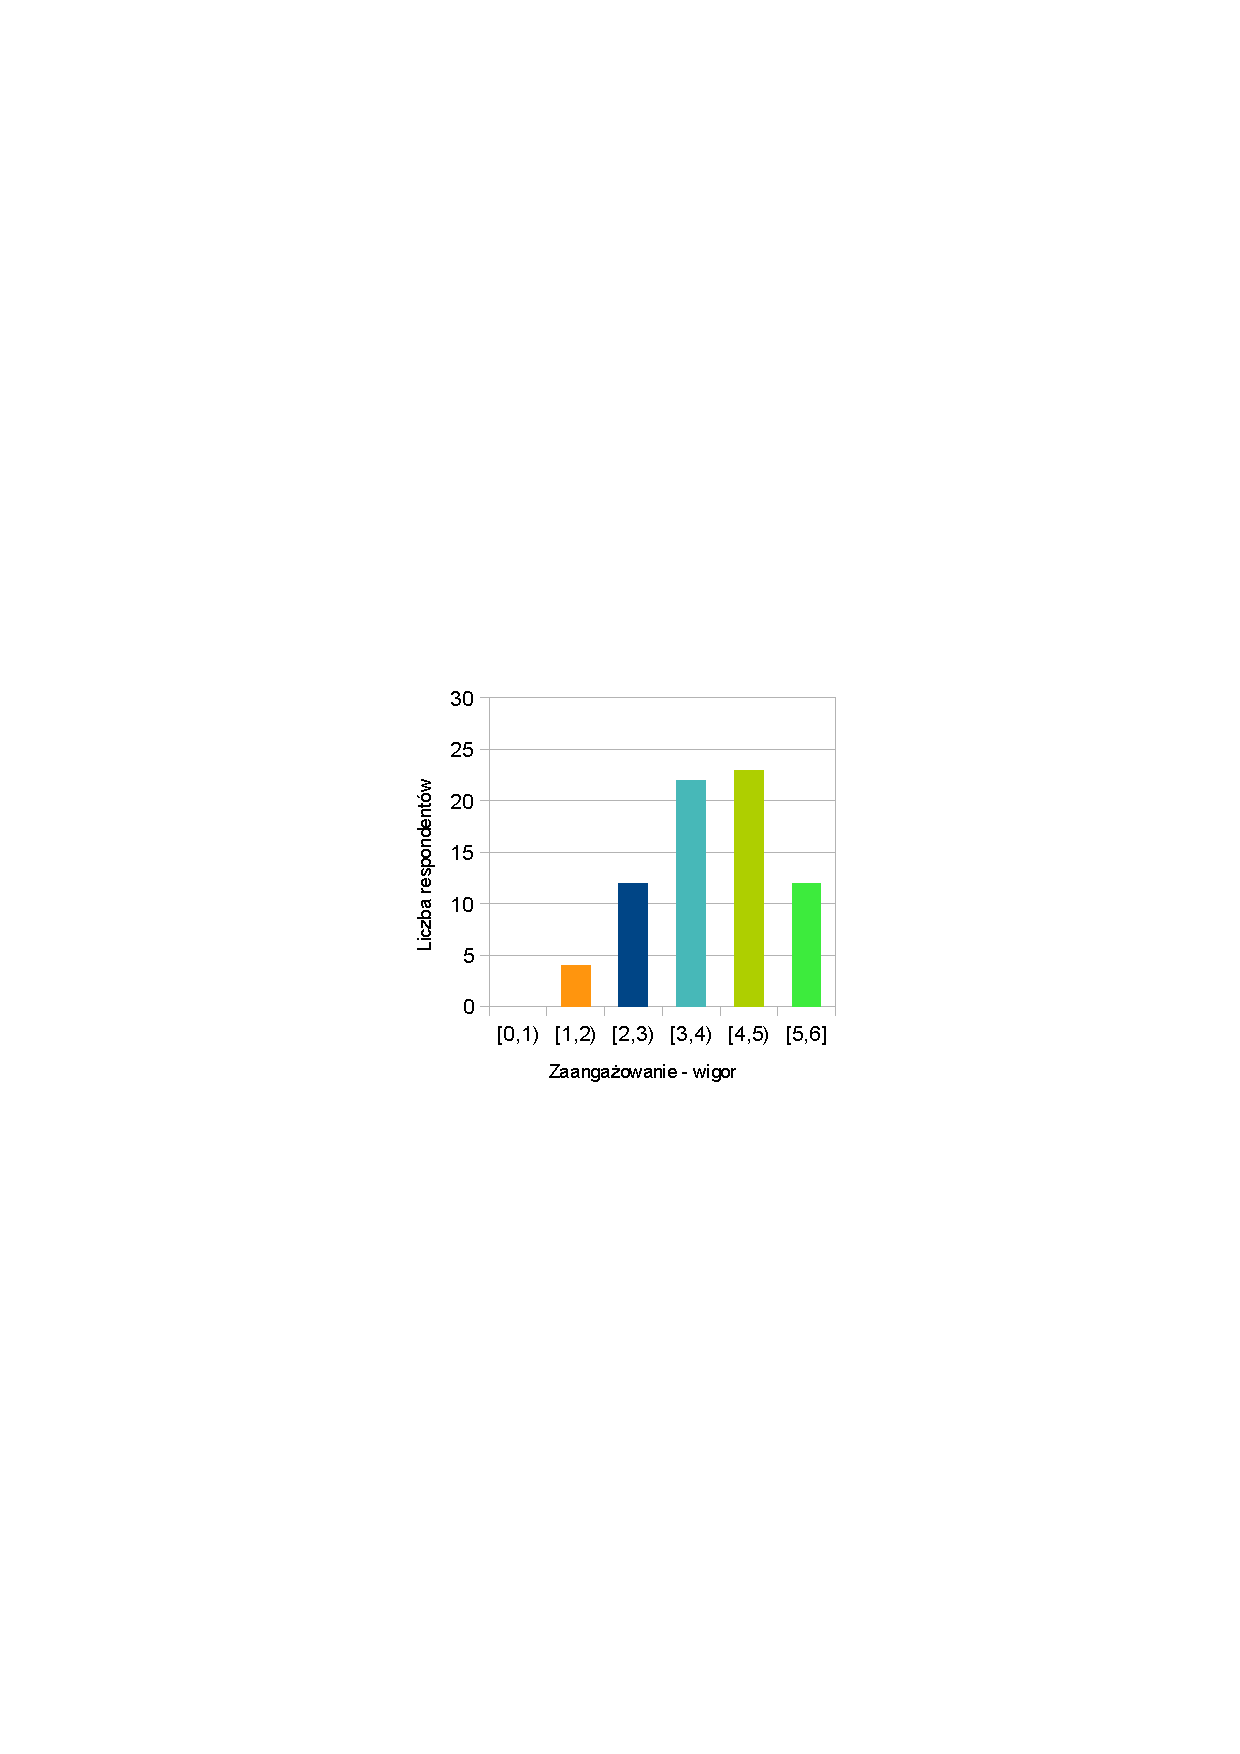
\includegraphics[height=0.27\textheight]{eng-vigor}}
    \subfloat[Oddanie]{\label{fig:eng-dedication}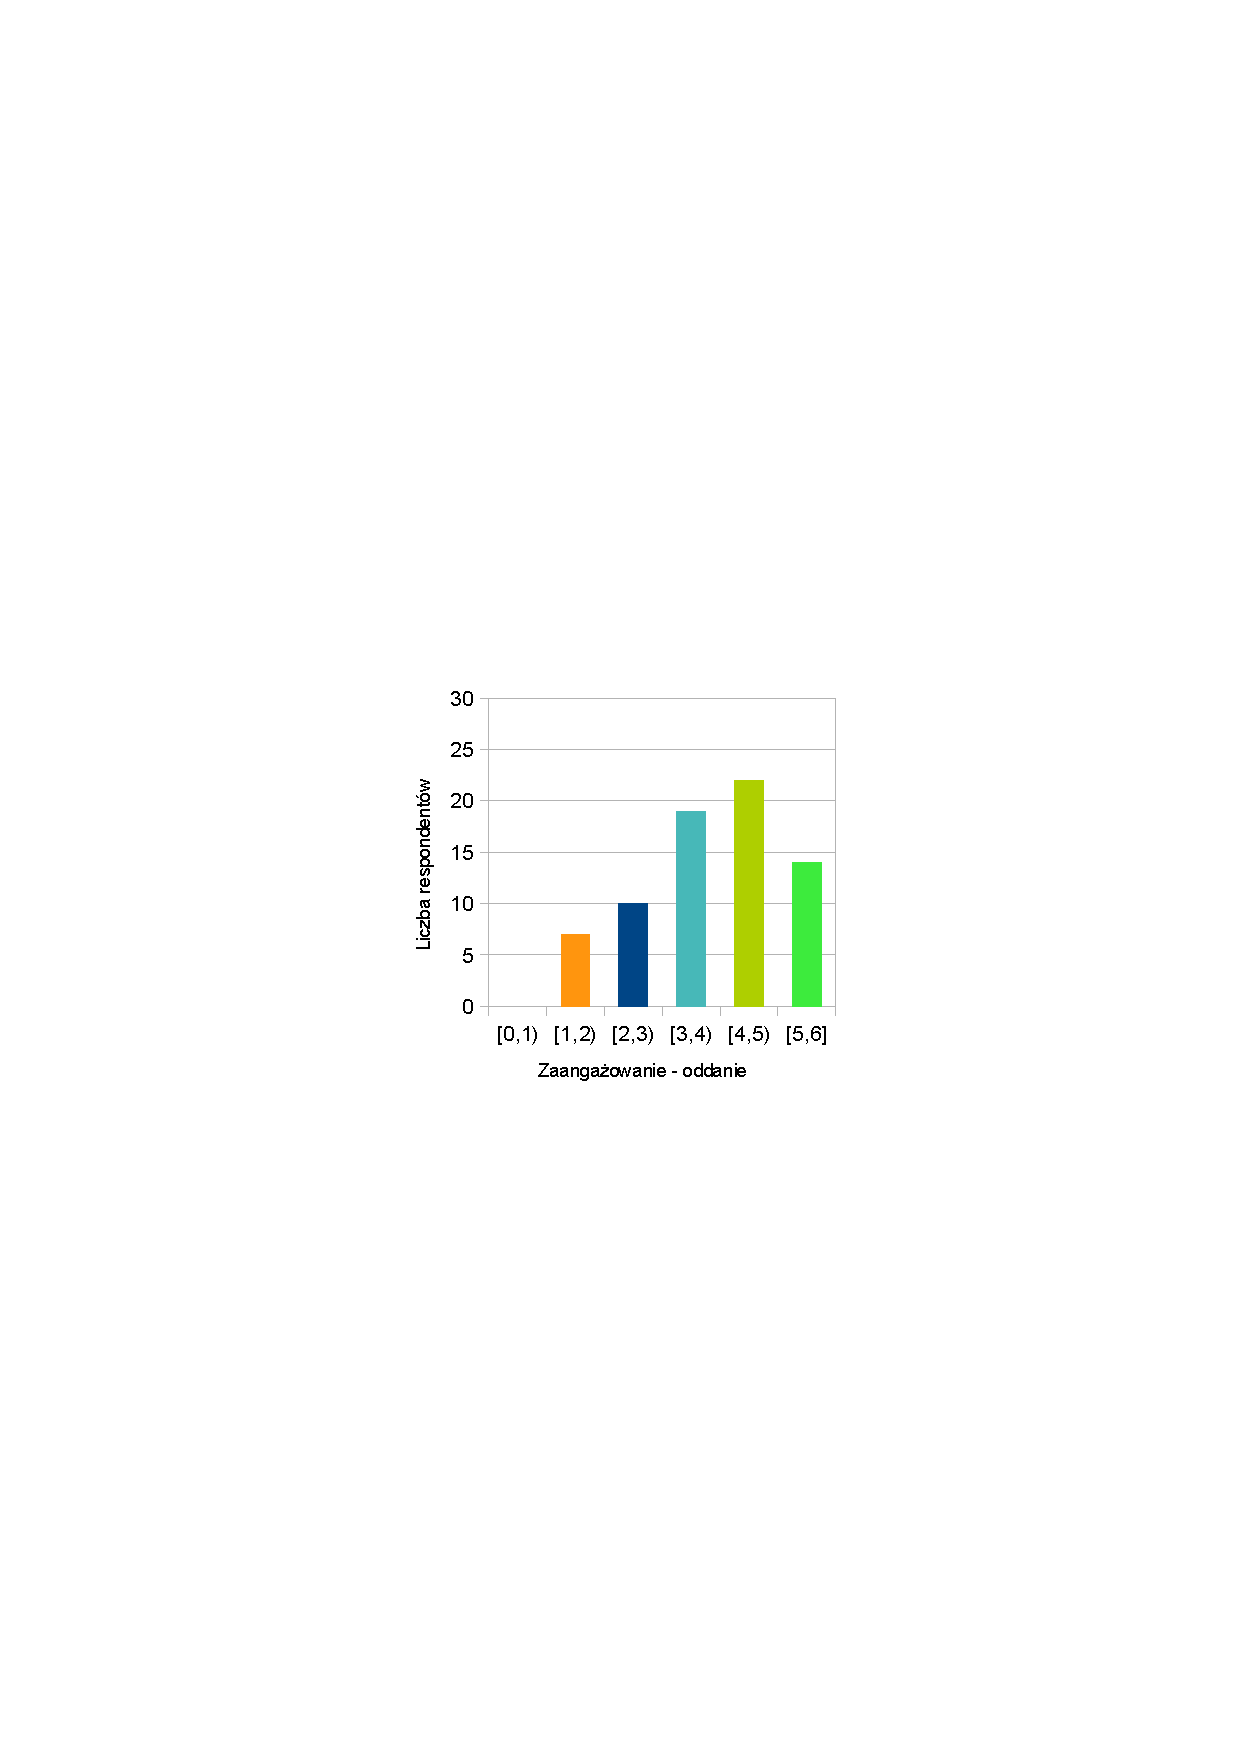
\includegraphics[height=0.27\textheight]{eng-dedication}}
    \\
    \subfloat[Absorpcja]{\label{fig:eng-absorption}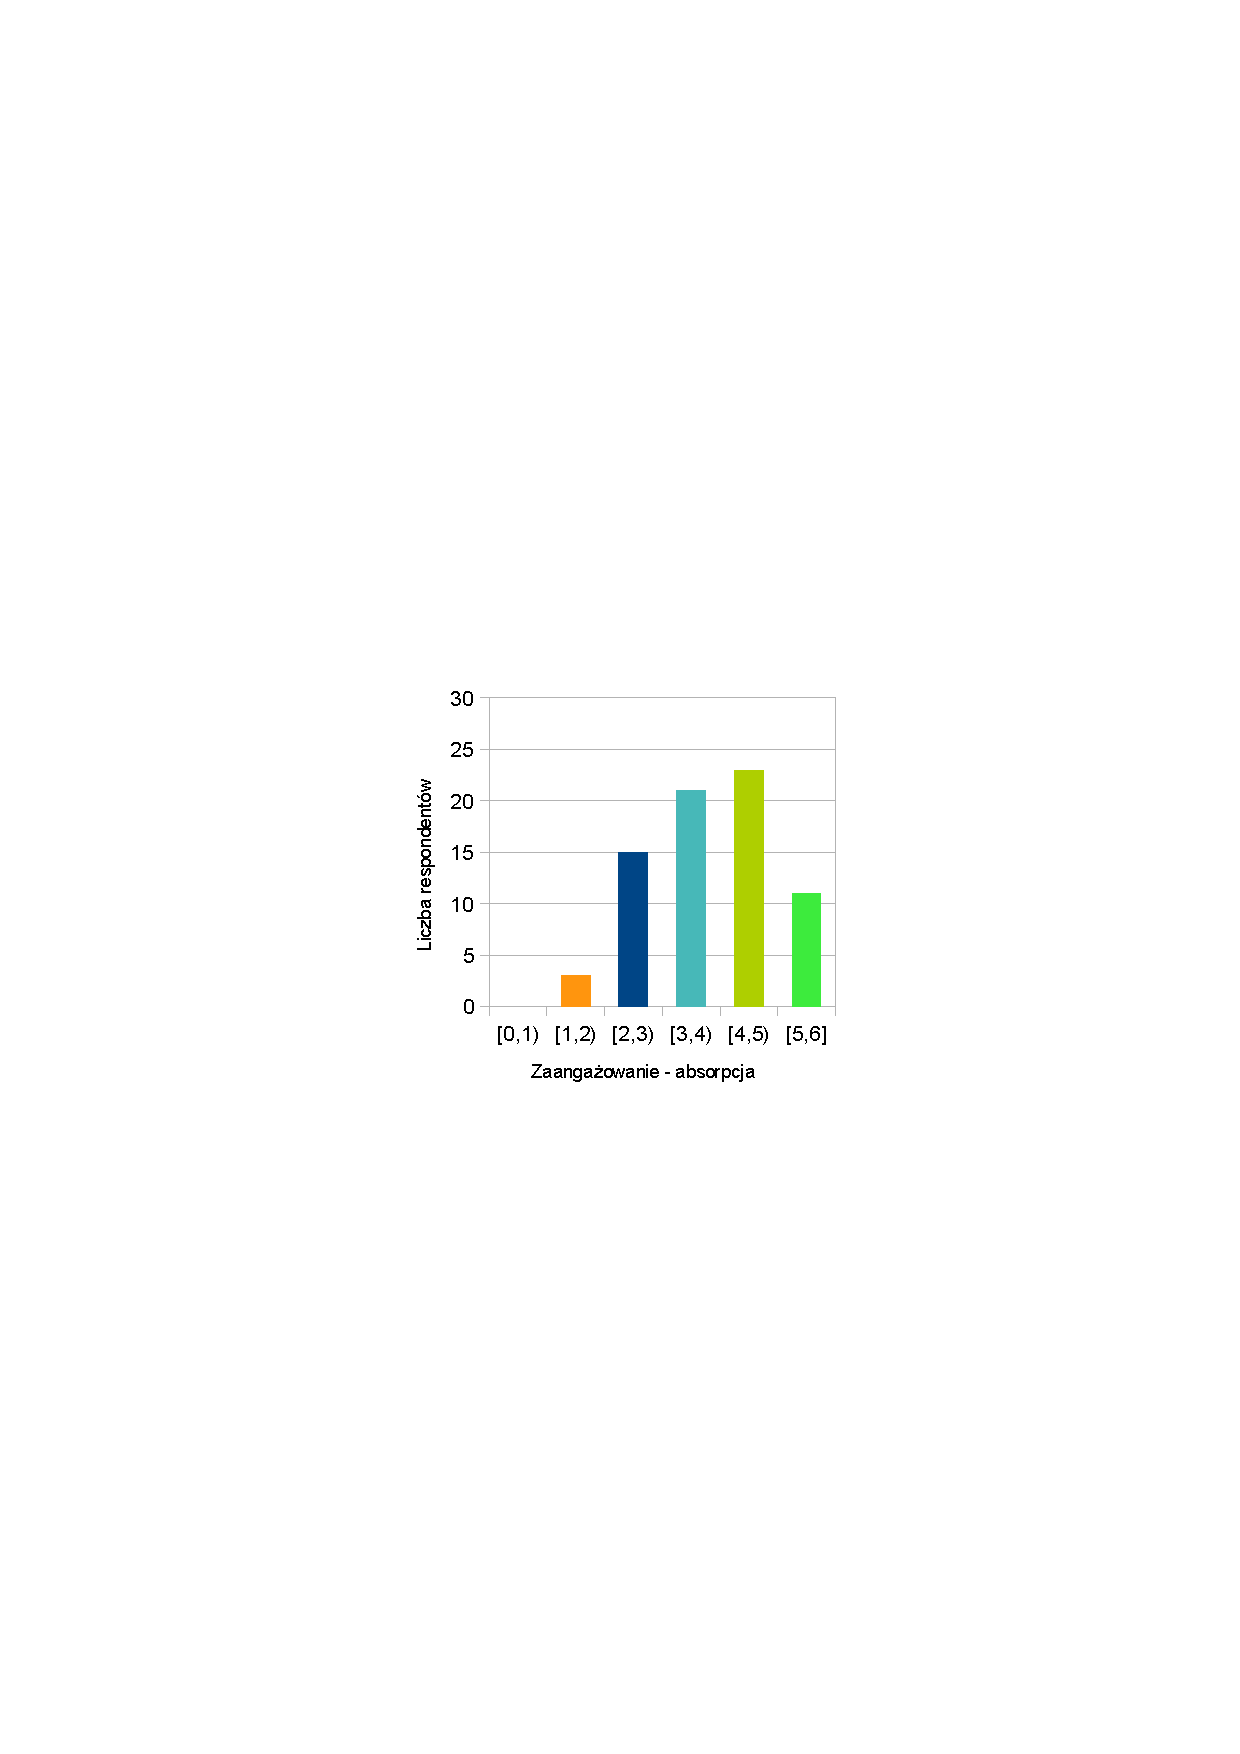
\includegraphics[height=0.27\textheight]{eng-absorption}}
    \subfloat[Zaangażowanie]{\label{fig:eng}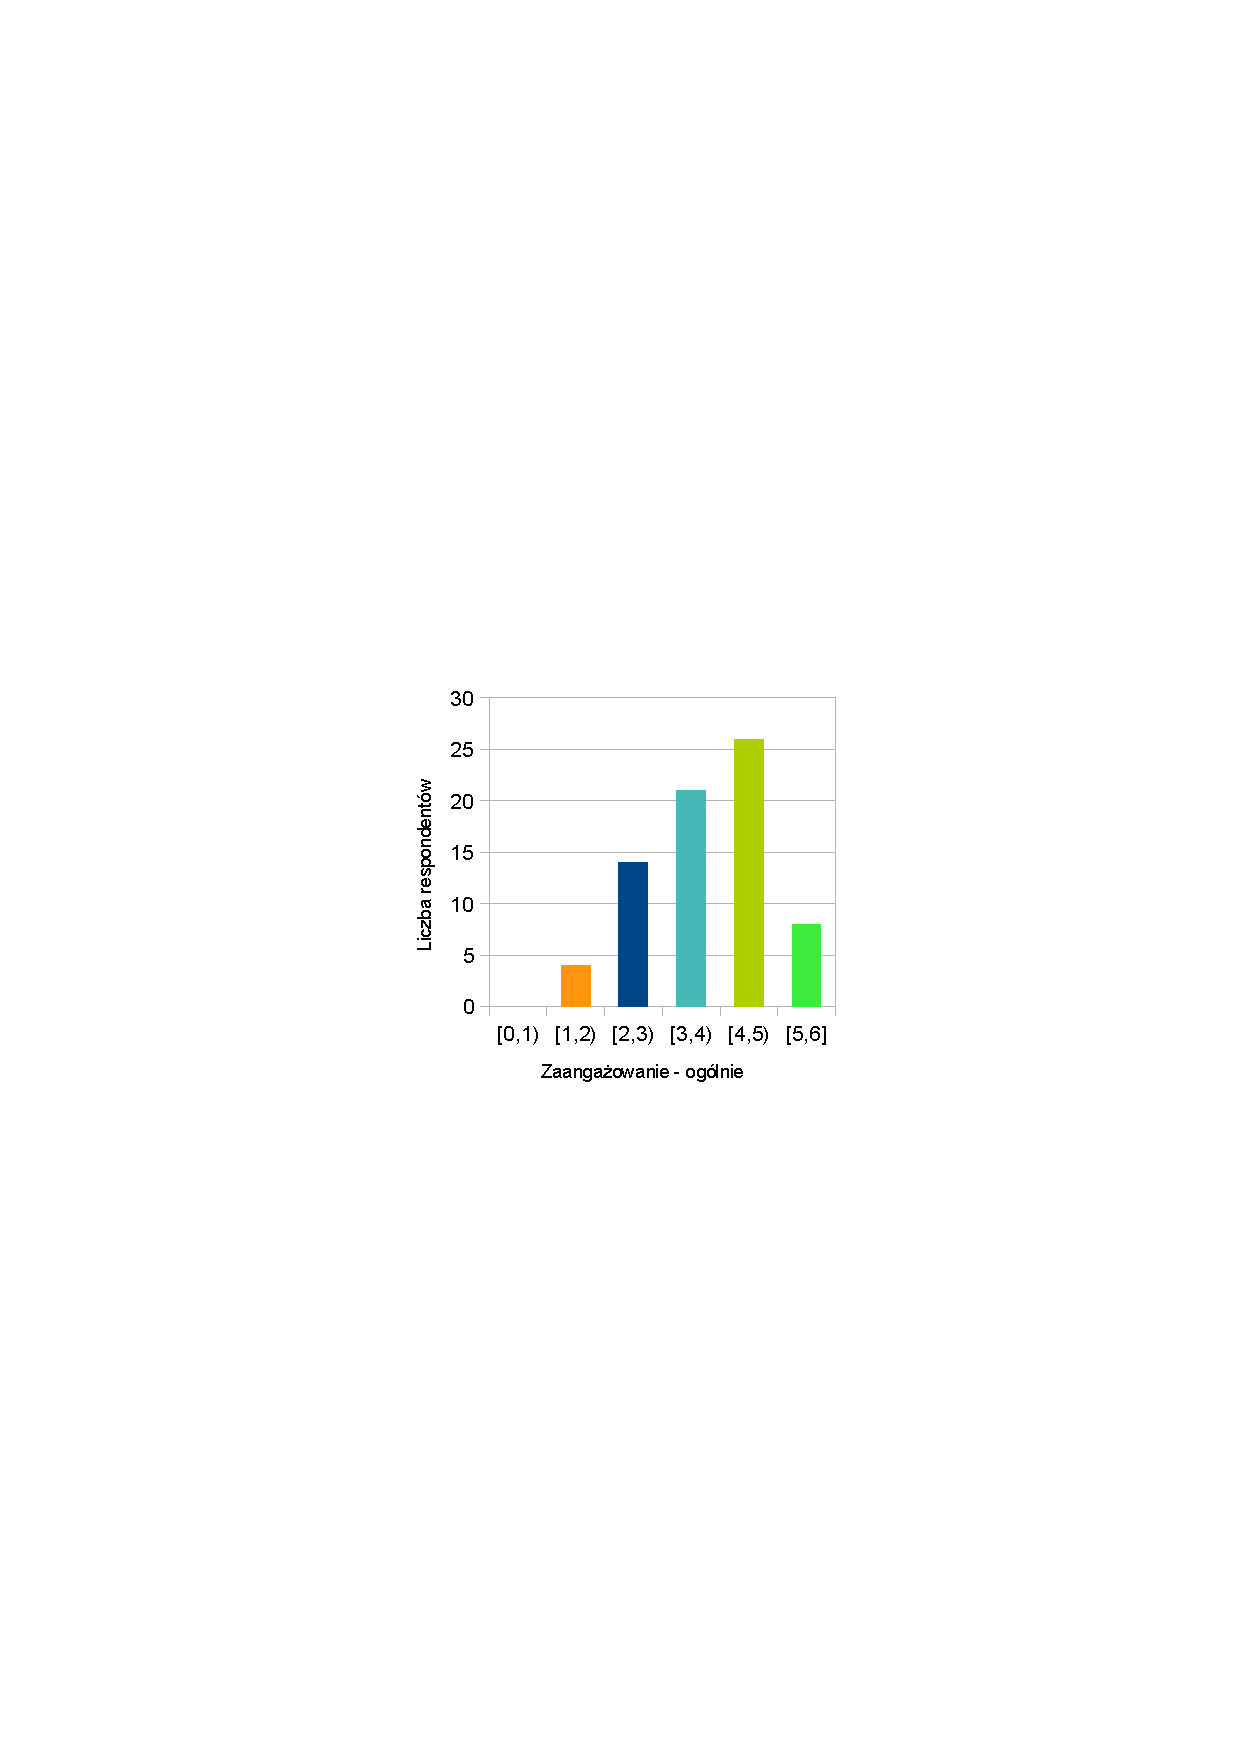
\includegraphics[height=0.27\textheight]{eng}}
    \caption{Histogramy dla \emph{UWES}}
\end{figure}

\begin{table}[h!]
\begin{center}
\begin{tabular}{l | c c c }
 & Wigor & Oddanie & Absorpcja \\ \hline \hline
Wigor & --- & 0,75 & 0,79 \\
Oddanie & & --- & 0,69 \\
Absorpcja & & & --- \\
\end{tabular}
\end{center}
\caption{Korelacja dla wszystkich wymiarów \emph{UWES}}
\label{tab:uwes-correl}
\end{table}

\paragraph{Wigor.} Wartości dla \textit{wigoru} rozpoczynają się od 1,33 (przynajmniej raz w roku) i rozciągają do 5.5 (przynajmniej kilka razy w tygodniu lub codziennie). Średnia to 3,75 (przynajmniej kilka razy w miesiącu). Pierwszy kwartyl to 3, czyli co najwyżej 25\% osób czuje wigor w pracy mniej niż kilka razy w miesiącu. Mediana to 3,83, czyli co najmniej 25\% osób ma podobne odczucia kilka razy w miesiącu. Trzeci kwartyl to 4,67, czyli co najmniej 25\%
respondentów jest pełnych energii w pracy między kilka razy w miesiącu do raza w tygodniu. Kolejne 25\% to osoby, które czują zaangażowannie co najmniej raz w tygodniu i wiecej. Jeżeli spojrzymy na Rysunek \ref{fig:eng-vigor} widzimy, że aż dwie-trzecie badanych odczuwa zaangażowanie od kilku razy w miesiącu do raza w tygodniu. Osób, które mają takie emocje co najawyżej raz w roku jest bardzo mało (dokładnie 4). Za to osoby najbardziej pożądane, które odczuwają wigor w pracy co najmniej
kilka razy w tygodniu to jedna-szósta respondentów (12 osób).

Ochylenie standardowe o wartości 1,06 jest średnie i wskazuje na średni rozrzut odpowiedzi badanych. Natomiast alfa Cronbacha na poziomie 0,83 wskazuje na wysoką spójność odpowiedzi respondentów.

\textit{Wigor} wykazuje wysoką zależność z pozostałymi wymiarami (patrz Tabela \ref{tab:uwes-correl}): \textit{oddanie} -- 0,75 oraz \textit{absorpcja} -- 0.79. Wskazuje to na silne powiązanie między odczuwaniem tych emocji lub ich bliskość semantyczną.

\paragraph{Oddanie.} Odpowiedzi respondentów dla \textit{oddania} zaczynają się od 1,4 (przynajmniej raz w roku) do 6 (maksymalna wartość, co najmniej kilka razy w miesiącu). Średnia to 3,79 -- przynajmniej kilka razy w miesiącu. Pierwszy kwartyl jest na poziomie kilku razy w miesiącu (wartość 3). Z tego wynika, że jedna-czwarta badanych oddaje się pracy co najwyżej kilka razy w miesiącu. Mediana to 4 (kilka razy w tygodniu), czyli co najmniej 25\% osób ma podobne odczucia
między kilkoma razami w miesiącu, a jednym razem w tygodniu. Trzeci kwartyl jest na poziomie kilku razy w tygodniu. Porównując z medianą widzimy, że co najmniej jedna-czwarta respondentów odczuwa oddanie w pracy przynajmniej kilka razy w tygodniu. Porównując te miary z Rysunkiem \ref{fig:eng-dedication} można dodać, że ok. jedna-trzecia badanych jest dumna z pracy i widzi sens swojej pracy między kilkoma razami w miesiącu, a jednym razem w tygodniu. Za to ok.
jedna-szósta ma analogiczne odczucia co najmniej kilka razy w tygodniu, a tylko 7 osób tylko kilka razy w roku.

Odchylenie standardowe jest na poziomie 1,21 (średnio-wysokie), co wskazuje na średnią różnorodność odpowiedzi respondentów. Alfa Cronbacha wynosi 0,9 i wskazuje na wysoką spójność w odpowiedziach badanych.

Natomiast korelacje z Tabeli \ref{tab:uwes-correl} (z \textit{wigorem} -- 0,75, z \textit{absorpcją} -- 0,69), podobnie jak z \textit{wigorem}, wskazują na dużą zaleśność między wymiarami lub podobieństwo semantyczne.

\paragraph{Absorpcja.} \textit{Absorpcja} przyjmuje wartości od 1,17 (przynajmniej raz w roku) do 5,83 (przynajmniej kilka razy w roku lub codziennie). Średnia wynosi 3,76 (przynajmniej kilka razy w miesiącu). Pierwszy kwartyl (wartość 3) wskazuje, że ok. 25\% respondentów wciąga się w prace co najwyżej raz do roku. Mediana na poziomie 3,5 pokazuje, że co najmniej 25\% osób odczuwa absorpcję w pracy kilka razy w miesiącu. Natomista trzeci kwartyl na poziomie
4,67 oznacza, że co najmniej 25\% ma podobne emocje w pracy przynajmniej raz w tygodniu, jak nie częściej. Patrząc na Rysunek \ref{fig:eng-absorption} można dodać, że ok. jedna-trzeciej badanych czas w pracy ucieka nie wiadomo kiedy co najmniej kilka razy w miesiącu, jak nie raz w tygodniu. Natomist tylko 3 osoby mają takie odczucia co najwyżej raz w roku. Z drugiej strony, tylko 11 osób czuje podobnie przynajmniej kilka razy w tygodniu.

Odchylenie standardowe jest średnie i wynosi 1,1 z czego wynika, że rozrzut odpowiedzi wśród respondentów jest ani wysoki ani niski. Natomiast alfa Cronbacha jest bardzo wysoka i wskazuje na wysoką rzetelność tego wymiaru.

Co do korelacji z Tabeli \ref{tab:uwes-correl} to jest podobnie jak poprzednimi wymiarami, jej wartości są bardzo wysokie: z \textit{wigorem} -- 0,79, z \textit{oddaniem} -- 0,69. Tak jak już było wspomniane wyżej wskazuje to na wysoką współżależność między wymiarami lub na ich semantyczną bliskość.  

\paragraph{Zaangażowanie ogólne.} Wartość minimalna to 1,47 (przynajmnie raz w roku), a maksymalna 5,83 (przynajmniej kilka razy w tygodniu). Pierwszy kwartyl to 3 (przynajmniej kilka razy w miesiącu), mediana 3,5 (także przynajmniej kilka razy w miesiącu)a, a trzeci kwartyl to 4,53 czyli kilka razy w tygodniu. Oznacza to, że mniej niż 25\% badanych odczuwa \textit{zaangażowanie ogólne} rzadko (co najwyżej raz w miesiącu). Więcej niż 25\% (patrząc na Rysunek \ref{fig:eng} można
doprecyzować że ok. jedna-trzecia) -- często czuje zaangażowanie
(od kilku razy w miesiącu do jednego w tygodniu), a kolejna ponad jedna-czwarta grupy -- bardzo często (co najmniej raz w tygodniu). Analizując dodatkowo histogram na Rysunku \ref{fig:eng} widzimi, że niewiele osób odczuwa zaangażowanie co najwyżej raz w roku (4 osoby) oraz niewiel osób odczuwa je bardzo często (8 osób, co najmniej kilka razy w tygodniu).

Rozrzut w danych jest średnio-niski, na co wskazuje odchylenie standardowe na poziomie 1,02. Natomiast alfa Cronbacha jest bardzo wysoka i wynosi 0,94, czyli cały test jest bardzo spójny jeżeli chodzi o badany aspekt pracy.

